\documentclass[a4paper]{article}
\usepackage[utf8]{inputenc}

\usepackage{amsmath}
\usepackage{amsfonts}
\usepackage{mathtools}

\usepackage{titling}
\usepackage[colorlinks]{hyperref}
\usepackage{graphicx}
\usepackage{listingsutf8}
\usepackage{xcolor}

\usepackage{float}

\usepackage[style=numeric]{biblatex}
\addbibresource{project.bib}

\setlength{\parindent}{0pt}
\setlength{\parskip}{\baselineskip}

\definecolor{codegreen}{rgb}{0,0.6,0}
\definecolor{codegray}{rgb}{0.5,0.5,0.5}
\definecolor{codepurple}{rgb}{0.58,0,0.82}
\definecolor{backcolour}{rgb}{0.95,0.95,0.92}

\lstdefinestyle{mystyle}{
    backgroundcolor=\color{backcolour},   
    commentstyle=\color{codegreen},
    keywordstyle=\color{magenta},
    numberstyle=\tiny\color{codegray},
    stringstyle=\color{codepurple},
    basicstyle=\ttfamily\footnotesize,
    breakatwhitespace=false,         
    breaklines=true,                 
    captionpos=b,                    
    keepspaces=true,                 
    numbers=left,                    
    numbersep=5pt,                  
    showspaces=false,                
    showstringspaces=false,
    showtabs=false,                  
    tabsize=2
}
\lstset{style=mystyle}

\newcommand{\subtitle}[1]{
    \posttitle{\par\end{center}\begin{center}\large#1\end{center}\vskip0.5em}
}

\DeclarePairedDelimiter{\ceil}{\lceil}{\rceil}
\newcommand{\R}{\mathbb{R}}
\renewcommand{\vec}[1]{\mathbf{#1}}

\title{\textbf{FYS-STK3155 Project 3}}
\subtitle{\url{https://github.uio.no/tobiala/FYS-STK3155-Project-3}}
\author{Severin Schirmer, Tobias Laundal \& Didrik Sten Ingebrigtsen}
\date{December 2020}


\begin{document}

\maketitle

\begin{abstract}
Property estimation based on observations is important in many fields. In this paper, we discuss a simple formulation of that problem, namely predicting the mass of a particle moving in a force field. We try to solve the problem using four different neural network architectures based on convolution and recurrence. Convolutional networks are known to handle spatial relations well, while recurrent networks should handle the temporal aspect well. The problem has a clear temporal and spatial part, so our initial hypothesis was that a model needed to be able to handle both in order to perform well. We used synthetic data generated by simulating experiments in stochastic force fields. In order to force the models to learn the general behaviour of particles in the fields, they only see each data point once during training and are tested on unseen data.

While little effort was put into tuning the models, we found that all models are able to solve the problem to a certain extent. The recurrent convolutional networks performs best overall, with an $R^2$ score of $0.461$. The difference between the different model architectures is less than anticipated, with dense and convolutional models achieving scores of $0.373$ and $0.408$ respectively. 
\end{abstract}

\section{Introduction}
% Motivation
It can often be useful to estimate the properties of an object in the real world, through observing how they react to outside forces. Giving a robotic system an idea of how heavy an object is before attempting to lift or push it, can aid in it performing a number of tasks faster and with higher precision. Finding the charge of a particle by observing its deflection when it moves through a magnetic field, has several upsides to more direct approaches \cite{dust_particle}. We look at estimating the mass of a particle from its trajectory through a force field, as this is a simple formulation of the same fundamental problem of predicting hidden properties. Results to this problem should hopefully generalize to the other similar problems.

% Objective and our approach
In this project we investigate if it is possible to estimate the mass of a particle given a force field and its trajectory through it using neural networks.  All our data is synthetic and generated from simulating experiments.  For each experiment, we draw a random mass for the particle and generate a random scalar potential field using perlin noise. We derive a vector force field from the scalar field by taking the gradient, and use this to simulate the trajectory of the particle. The simulation is itself discrete, and we will refer to each iteration of a simulation as a simulation step. The data available to our models is a scaled down version of the scalar potential field and some positions sampled from the trajectory, which we call time steps.

We designed the problem to gain more insight into convolutional neural networks and recurrent neural networks. Using the stated problem, we explore how convolution aids in interpreting spatial information from the scalar potential, and how recurrence may utilize more temporal information from the trajectory. We do not provide a benchmark to compare our results against, but we discuss what a possible non-machine-learning solution to this problem might look like.

The report begins with a more formal introduction to our problem, and to the theory behind our data generation. We then discuss the theory behind the different model architectures we used, before covering loss functions and functions to evaluate model performance. This is followed by explanations of the implementation of both data generation and the models.  Finally, we present the results along with our discussion and conclusion.


\section{Theory}

\subsection{Problem and generation of data}
\label{subsec:theory-data-gen}
Since we haven't been able to find a dataset of appropriate type, and the problem is easy to simulate, we have made a synthetic dataset. Here, we work with a high resolution field, $256\times256$, generated pseudorandomly and numerically solve a set of differential equations governing the particle's position. We down-sample the field spatially, making a lower resolution image $32\times32$, and the simulated trajectory temporally, only keeping every tenth simulation step. When we later refer to time steps, it is these subsampled steps we have in mind, not all the later discarded simulation steps.

Because we down-sample, and because the particle's velocity isn't explicitly given to our models, we have a partially observed problem, with the velocity as a hidden state. For the model to perform well, we hypothesise that it will need to estimate this hidden state. We also believe the spatial dimension of the problem is non-trivial. The goal is to construct a model that can deal both with the spatial and temporal complexity. We estimated the importance of the two parts, by seeing how well a model suited mainly for only one of the two parts is able to solve the problem.

Our experiments start with a stochastic mass and scalar field. The mass is drawn from a continuous uniform distribution with bounds 0.1 and 1. The scalar potential field is generated with Perlin noise explained below. Given a scalar potential field $\phi(x, y)$, we derive the force field  $\vec{F} = - \nabla\phi$. With a particle mass $m$ and position $\vec{r}$, Newton's second law gives us the acceleration of the particle $\vec{a} = \frac{\vec{F}(x, y)}{m}$. In general, the particle's position $\vec{r}$ at time $t$ is given by the differential equations in equation \ref{eq:diff_particle}.

\begin{equation}
    \label{eq:diff_particle}
    \begin{split}
    \frac{\partial \vec{r}}{\partial t} = \vec{v} \quad
    \frac{\partial \vec{v}}{\partial t} = \vec{a} = \frac{\vec{F}(\vec{r})}{m} \\
    \end{split}
\end{equation}

When simulating the trajectory of the particle, which is part of the input to the models, we solve equation \ref{eq:diff_particle} numerically. The scalar and vector fields we simulate in are high resolution, and we may treat the time elapsed between each simulation step as arbitrarily small. We scale down the scalar field with a factor~$k=8$ before it is used by our models, in order to keep them somewhat small and force the model to infer some more aspects of the data . The scaled down scalar field, $\psi$, is then given by
equation \ref{eq:scale_down}.

\begin{equation}
    \label{eq:scale_down}
    \psi(x,y) = \frac{1}{k^2}
      \sum_{i=0}^k\sum_{j=0}^k \phi(kx + i, ky + j)
\end{equation}

For the time steps to be interpretable by convolution, we choose to encode them in fields of the same size as the down scaled potential fields ($32\times32$). One hot encoding the position of the particle decreases the accuracy of the position. Instead we use a method we have chosen to name four-warm encoding. The goal of four-warm encoding is to encode the position of the particle in a field of the same size as the scaled down scalar field without loosing any precision. The field is a grid, and for each of the four closest locations in the grid to the actual position, we assign the value $(1 - \left|\vec{r}_x - i\right|)(1 - \left|\vec{r}_y - j\right|)$, where $\vec{r}$ is the position of the particle and $i$ and $j$ are the x and y position of the location in the grid. This is visualized in figure \ref{fig:four-warm}. Four-warm encoding achieves our goal quite well as all positions are uniquely represented, except for the coordinates along the perimeter where only two points will be activated.

\begin{figure}
    \centering
    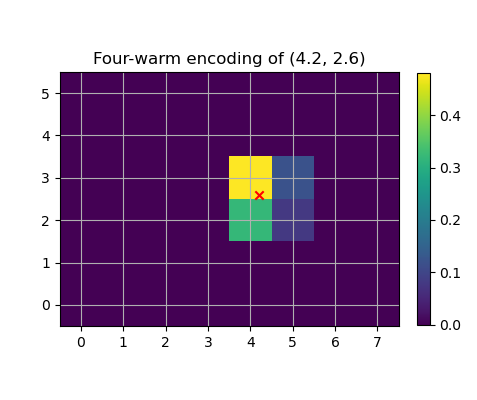
\includegraphics[width=0.8\textwidth]{Figures/four-warm-encoding.png}
    \caption{Illustration of the four-warm encoding. The red cross represents the exact
             position we wish to represent. The background coloring is the four-warm
             field. Notice that each square in the field represents one intersection in
             the grid. The field values in the four intersections closest to the red
             cross sum to one, and should accurately represent the position.}
    \label{fig:four-warm}
\end{figure}

The scalar fields used to simulate the forces acting on the particles needed to seem continuous and show a level of orderliness despite being random such that the particles would follow a path through the field without being thrown back and forth. With messy fields, e.g. white noise, the simulation step size has a bigger effect on how the particle moves. In order to achieve orderly but random fields we employed Perlin noise, a noise function created by Ken Perlin which has been widely used in video games to generate terrain and realistic looking textures \cite{perlin}. We employ them here to create coherent force fields with clear minima and maxima. 

Because our data is synthetic and this exact formulation of the problem is novel, we do not have a benchmark to compare our method to. The true values for the particle mass provides an ideal goal to reach for, but we have no realistic baseline to compare our model performance to. Given the exact same restrictions as our models have, with the field and particle position as input, one possible way to estimate the mass would be to simulate particles of different masses in the provided, scaled down field, and binary search for a mass which travels the same distance in the same amount of time steps. A solution like this does however assume knowledge of how the particle actually behaves, and would potentially not improve the estimate significantly over multiple time steps, as a lot of information is lost when down sampling the scalar field. An alternative solution is beyond the scope of this project and we have not taken the time to implement one.

\subsection{Model}
A good model needs to have some understanding of how the particle's mass and the field together accelerate the particle. Our problem is impossible to solve perfectly in just one time step, since the particle's mass is under-determined when the field is scaled down. Our hope is that the trajectory of the particle gives enough information to more precisely predict the mass. Our model needs to be able to both understand spatial and temporal relations. We have decided to use neural networks to solve this problem, because they have the capacity to deal with complex problems without much prior knowledge, and have separable modules to deal with both this spatial and temporal parts. Additionally we hope convolutional layers will help in understanding spatial relations of the data better than dense layers, and that a recurrent model will show improved understanding of the temporal data.

Since the data used to train is generated, and we therefore don't have to see the same data point more than once, overfitting is not an issue.

\subsubsection{Convolutional neural networks}
Convolutional neural networks have been the primary method in image recognition since 2012. They emerged from studying the visual cortex of cats and mimic how neurons are activated by certain areas of the visual field as opposed to neurons in densely connected layers which receive a signal from every input \cite{Geron}. Convolutional layers' edge in image recognition is their ability to detect spatial relations and structures in the input. Our previous project used simple dense layers to recognize images which therefore discarded important structural information about how the pixels relate to each other \cite{didsev}. For the network to understand the structure of the field we therefore use convolutional layers with the aim for the network to get a general understanding of how the position of the particle relates to the field. 

The mathematical operation of convolution combines two functions by weighting one with the other. This can be useful when interpreting sensor data or other signals. Given two functions $f$ and $g$, the definition of their convolution $f*g$ is given in equation \ref{eq:convolution} \cite{FYSSTK4155}. The convolution of one function with a weighting function may be used to smooth out noisy data or give some interpretation dependent on the value of the function along its domain.

\begin{equation}
    \label{eq:convolution}
    (f*g)(t) =
    \int_{-\infty}^{\infty} f(\tau)g(t - \tau) d\tau
\end{equation}

Convolutional layers in neural networks apply a very similar principle in order to pick up spatial structure in a preceding two-dimensional layer. The weighting is done by a kernel, which itself is a matrix. The kernel is moved along the axes of the preceding layer with specific strides. The output of the convolutional layer is given by each position of the kernel. For each position, the value is the weighted sum of the corresponding values in the preceding layer \cite{Geron}. The concept is described in figure \ref{fig:convolution}. Mathematically, if we let the preceding layer be given as a matrix $A \in \R^{n \times m}$, the kernel as a matrix $K \in \R^{a \times b}$ and the stride of the kernel be $s$ in both directions, the output of the convolution layer would be a matrix $C \in \R^{\ceil{s^{-1}(n - a + 1)} \times \ceil{s^{-1}(m - b + 1)}}$, where the values in $C$ are given as in equation \ref{eq:convolution_layer}. We have here not included a bias term, which may also be used. The process can also be generalized to apply to preceding layers of higher dimensions, and multiple channels. When using multiple channels, the kernel has different weights for each channel, but their weighted sums are summed in the output. A single convolution layer may also contain multiple independent kernels, such that the output from the layer has multiple channels.

\begin{equation}
    \label{eq:convolution_layer}
    C_{i,j} = \sum_{k=0}^{a} \sum_{l=0}^{b} K_{k,l} A_{si+k,sj+l}
\end{equation}

\begin{figure}
    \centering
    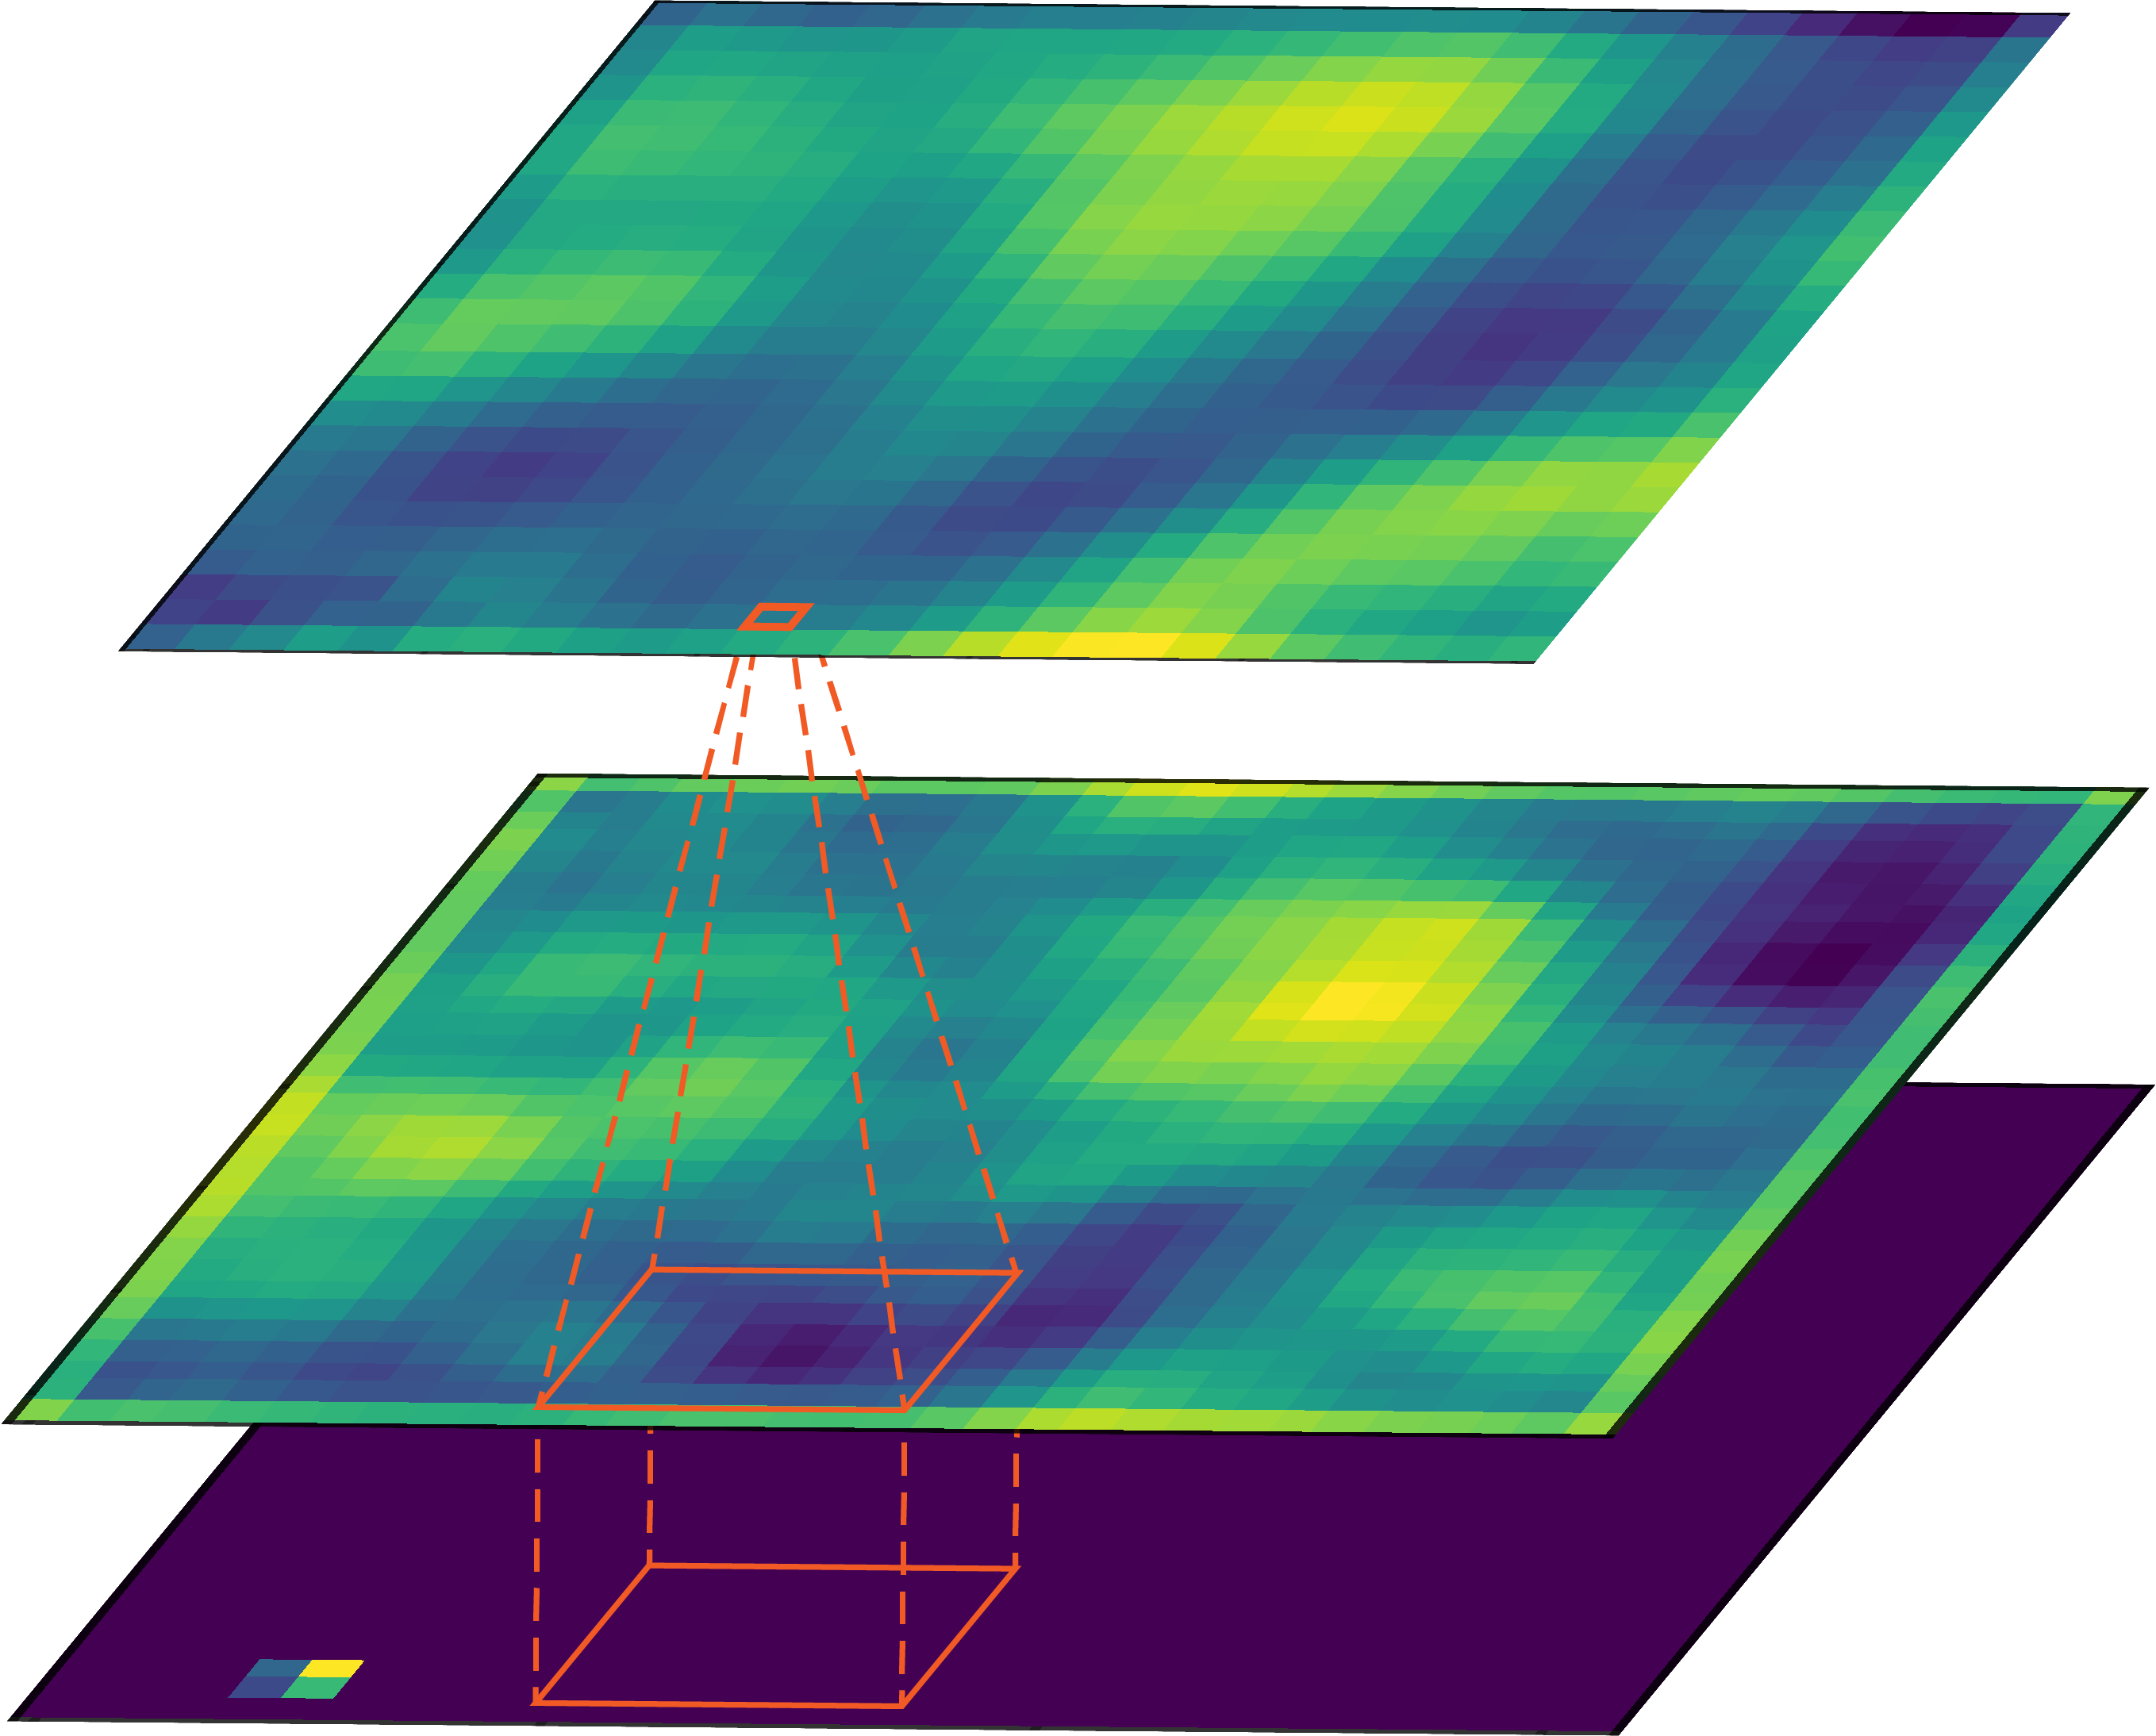
\includegraphics[width=0.8\textwidth]{Figures/Conv_model.png}
    \caption{Illustration of a convolutional layer in a neural network. The two bottom images are the input position and scalar field and the top is the output from a convolutional layer with a single filter. The red squares illustrate the convolution kernel and the corresponding output. Here the kernel has size 7x7.}
    \label{fig:convolution}
\end{figure}

\subsubsection{Recurrent neural networks}

A recurrent neural network (RNN) stores some node state in between time steps, so that information learned about the system can be built upon over time. There are several classes of RNNs, and we have chosen to use a Gated Recurrent Unit (GRU). We use GRU instead of a vanilla RNN method to prevent vanishing gradients. When training RNNs, errors propagate through several time step iterations of the same network and they quickly become very deep. This makes vanishing gradients occur much more frequently, and prevent gradient methods from effectively optimising the parameters for the data it was fed in anything but the last few time steps \cite{gru_vs_lstm}. GRUs deal with this problem by not overwriting the node states every time like conventional RNNs, but instead only add information to it. This keeps important information over several time steps \cite{gru_vs_lstm}.

Using GRU, the $j$'th activation $h_t^j$ at time step $t$, is calculated by

$$ h_t^j = (1 - z_t^j)h_{t-1}^j + z_t^j \tilde{h}_t^j $$

Here, $\tilde{h}_t^j$ is the activation candidate, found as

$$ \tilde{h}_t^j = \tanh{(W_h \vec{x}_t + U_h(\vec{r}_t \odot \vec{h}_{t-1}))^j} $$

$\odot$ is the Hadamard product, $W$ and $U$ are parameter matrices and $\vec{x}_t$ is the output from the previous layer. The update gate $z_t^j$ and reset gate $r_t^j$, which together decides which parts of the state to preserve, and which to replace with new information, are formulated as follows:

\begin{align*}
z_t^j &= \sigma (W_z \mathbf{x_t} + U_z \mathbf{h_{t-1}})^j \\
r_t^j &= \sigma (W_r \mathbf{x_t} + U_r \mathbf{h_{t-1}})^j
\end{align*}

Another option for a class of RNNs with a similar solution for vanishing gradients to GRU is long short-term memory (LSTM). Because it is slightly more complex, and GRU seems to perform comparatively well \cite{gru_vs_lstm}, we have opted to work with GRU here.

\subsubsection{Convolutional recurrent neural network}
\label{subsubsec:crnn_theory}

In order to combine the powers of the spatially aware CNN, with the temporally aware RNN, we need to stack the network with the RNN on top of the CNN. For each time step, the model will then process the input fields through the convolution layer, before they are passed on to the GRU. Training a model with this kid of architecture can be done in several ways. We will outline how this can be done with and without penalizing the model for how good predictions the intermediate outputs from the recurrent units are. Assessing the intermediate outputs of the model forces it to try to keep track of a best prediction throughout the time steps. Training may then be done with the following steps.

\begin{enumerate}
    \item Give the CNN one time step as input, and pass the CNN output to the RNN. Store the RNN state and prediction.
    \item Evaluate the loss function, and back propagate the loss through the all the steps made up until this point, both CNN and RNN.
    \item Update parameters accordingly.
    \item Repeat steps 1 - 3 for each time step in the simulation. Pass the RNNs previous state back to it in each step.
\end{enumerate}

This gives us a new prediction for each time step, making it easy to see how many time steps we need to converge on a solution. Predictions may be made after only a few time steps and it is possible to analyse the way the RNNs state stores information. The big problem with this algorithm is that the model will be told for each time step to give the same output. Initially, this might make it hard for the model to trust the recurrent state at all, and we suspect the training will end up being sub-optimal. We have not tried to solve this problem directly in this project. Instead, we use the following algorithm to evaluate and train the network.

\begin{enumerate}
    \item Give the CNN all the time steps one after another, and save the results as a large tensor.
    \item Pass this output (with all the different time steps combined) to the RNN.
    \item Back propagate the error through all the steps made and store the changes for the CNN and RNN
    \item Update parameters of CNN and RNN with the mean of the stored changes.
\end{enumerate}

This algorithm runs through all the time steps before making a prediction, and before back propagation. This hopefully emphasises how important the RNN state is during training, and prevents fitting too much to each sample. However, this also prevents the model from making sane predictions partway through the time steps. It is still possible to extract predictions after each time step, but since the model isn't trained to make these accurate, they might not be that informative. This last framework for building a model is called many-to-one, since it takes in many time steps and only gives one prediction, while the first framework is called many-to-many.

\subsection{Loss functions and model assessment}
\label{subsec:loss_theory}
Because we have a regression problem, mean squared error (MSE) seems like a good candidate for a loss function. A property of MSE is that the error doesn't scale with the size of the actual data. Using MSE will therefore make the model care less about being $5\%$ off if the particle has a low mass, than it would if it was big. To combat this, we have tried using mean absolute percentage (MAP) as our loss function in addition to MSE. MAP is defined in equation \ref{eq:MAP}, and gives us relative instead of absolute error. We have also tried the Huber loss function, which is exactly like MSE up to some parameter value difference between prediction and target, before it is linear instead of quadratic.

\begin{equation}
    \label{eq:MAP}
    \mathrm{MAP} = 100 \sum_i \frac{\left| y_i - \tilde{y}_i \right|}{y_i}
\end{equation}

We did some tests with these loss functions, and found that variation in between different training runs with the same loss function seemed just as high as between runs with Huber and MSE. MAP however, performs noticeably worse. Testing the performance of these loss functions rigorously wasn't the main point of the report, and finding estimates for mean and variance for performance with different loss functions would be computationally expensive. Instead we have visualized, in figure \ref{fig:loss-visualisation}, how the different loss functions would penalize predictions for different particle masses. We have used Huber with a $\delta$-parameter of $0.2$ throughout the project.

\begin{figure}
    \centering
    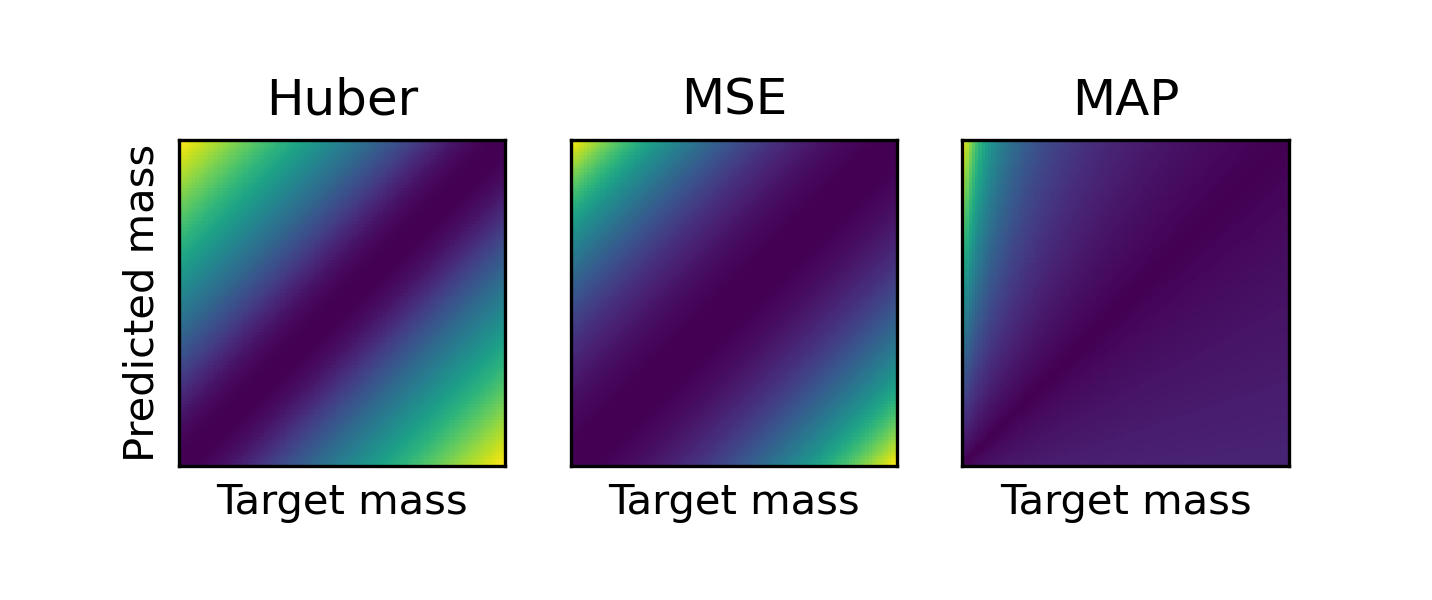
\includegraphics{Figures/loss_visualisation.png}
    \caption{The three loss functions we have considered. Each plot has an independent color scale. Here, the loss is lowest (dark blue) near the diagonal from bottom left to top right. This is the diagonal where our prediction matches our target. Huber and MSE looks very similar, because the $\delta$-parameter determining how large the L2 error must be before the loss changes from quadratic to linear is $0.2$. MAP looks quite different, with the loss getting highest for being furthest away in L2 distance from the lowest possible masses.}
    \label{fig:loss-visualisation}
\end{figure}

\subsubsection{Assessment}

MSE, MAP and Huber are probably not the best metrics for assessing how good a model is. As is confirmed later in the results section, they are all metrics where it is difficult to see the difference between a model that only predicts the average, and one that makes poor predictions that still share some properties with the actual masses. A metric that does say something about correlation is $R^2$. It is defined as

\begin{equation*}
    R^2 = 1 - \frac{\sum_i (y_i - \tilde{y}_i)^2}{\sum_i (y_i - \bar{y})^2}
\end{equation*}

If the predictions are all the average of the actual masses, the $R^2$ score is $0$, if they are all the same it is $1$, and if they have some sort of negative correlation the score is negative. It's not perfect, but it can help us take into account both the variance and mean of the predictions, as well as what kind of correlation they have to the target. If we however just want to look at the correlation, there is a more powerful metric. The Pearson correlation coefficient is the scaled covariance between two variables. It gives a scale from $-1$ to $1$, which says how good of an indicator the first variable is of the other. If it is $1$, it doesn't necessarily mean they are the same, but that a linear function exists that gives a mapping between them. The Pearson correlation coefficient is defined as

\begin{equation*}
    \rho_{X,Y} = \frac{\mathrm{Cov}{(X,Y)}}{\sigma_X \sigma_Y}
\end{equation*}

\section{Implementation}

\subsection{Data generation}
Our data is generated following the steps outlined in section \ref{subsec:theory-data-gen}. For each experiment, we generate a field using Perlin noise, choose a mass and simulate a particle of that mass moving in the field. The Perlin noise generation is done by the Python package "noise" \cite{pypi-noise}. The package takes a few arguments for tweaking the appearance of the noise. We tweaked these to give a field which seemed reasonable smooth. One configuration of arguments gives one, infinite, field. For each experiment, we pick two floating point numbers independently from a uniform distribution in the interval from $10^{-5}$ to $10^{5}$, and use these as x and y offsets for a unit square in our Perlin noise field. This should give virtually limitless number of finite fields, and in any case more fields than our models would be able to memorize. To prevent particles from escaping the fields during simulation, we convert the field to a trap. This process is explained in listing \ref{lst:trap}.

\begin{lstlisting}[
  caption={Function which transforms our fields so the particles doesn't escape during simulation. The \lstinline{trap} variable has a bowl like shape with a flat bottom, and an edge with height 1. In the last line, the original field is weighted down near the edges and summed with the bowl-like field.},
  float,
  language=Python,
  label={lst:trap}
]
def trap(field, flatness=25, safety=1.1):
    """Convert the field to a trap

    :param field: Field to turn into a trap. Ideally with values
                  from -1 to 1.
    :param flatness: Controls how "wide" the edges of the bowl are
    :param safety: Height of the edges
    :return: The field turned into a trap
    """
    width, height = field.shape
    x, y = np.meshgrid(np.linspace(-flatness, flatness, width),
                       np.linspace(-flatness, flatness, height))
    trap = np.max([np.exp(np.abs(x) - flatness),
                   np.exp(np.abs(y) - flatness)], axis=0)
    return (1-trap) * field + safety * trap
\end{lstlisting}

With the field ready, we draw a mass from an uniform distribution between $0.1$ and 1. We then have enough data to solve the differential equations given in equation \ref{eq:diff_particle} numerically. This process is in essence a loop over the number of simulation steps we wish to perform, where each step is performed by the function given in listing \ref{lst:simulation-step}. Figure \ref{fig:fields} shows three fields, with their gradient vectors and a simulated trajectory over 150 simulation steps. We have not validated our fields or simulations except verifying that the fields, vectors and trajectories in this plot corresponds well. 

\begin{lstlisting}[
  caption={The function which performs each step in the numerical solving of equation \ref{eq:diff_particle} for simulating a particle in a field.},
  float,
  language=Python,
  label={lst:simulation-step}
]
def next_position_velocity(force_field, mass, position, velocity):
    r"""Calculate the position and velocity in the next time step.

    The x and y indices of the force vectors in the fields
    are assumed to apply in all positions
    :math:`(x', y') \in [x, x+1) \times [y, y+1)`.

    :param force_field: A force field as 3d, matrix-indexed array
                        of shape (y, x, 2).
    :param mass: Mass of the particle.
    :param position: Current position of the particle, as an array
                     of cartesian coordinates ``(x, y)``.
    :param velocity: Current velocity of the particle in the given
                     field, as an array like ``position``.
    :returns: The next position and velocity of the particle, as
              tuple of cartesian coordinate arrays.
    """
    x, y = position
    acceleration = force_field[int(y), int(x)] / mass

    next_vel = velocity + acceleration
    next_pos = position + next_vel

    return next_pos, next_vel
\end{lstlisting}

\begin{figure}
    \centering
    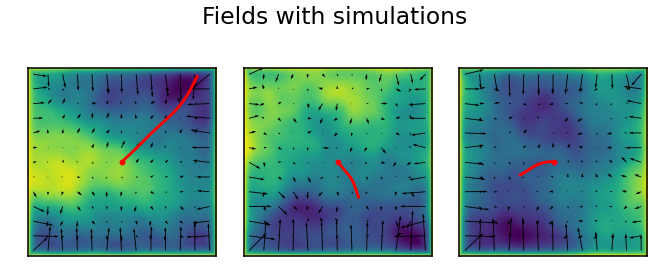
\includegraphics[width=\textwidth]{Figures/fields.png}
    \caption{Three randomly generated fields, with the trajectory of a particle with mass $0.9$ simulated over 150 simulation steps. Yellow color indicates high values in the underlying field, while dark purple is low values. The values range from $-1$ to 1.}
    \label{fig:fields}
\end{figure}

The data is generated while running the code and we do not store the data sets to disk, but can still reproduce the same data by setting the same seed for our pseudo-random number generators. We do however, encode the trajectory differently for the different models. In our feed-forward models, we sum the four-warm encoding of each the position in each time step to one field representing the whole trajectory, while our recurrent models receive each four-warm encoded position separately. These methods for encoding the trajectory are illustrated in figure \ref{fig:position_input}.

\begin{figure}
    \centering
    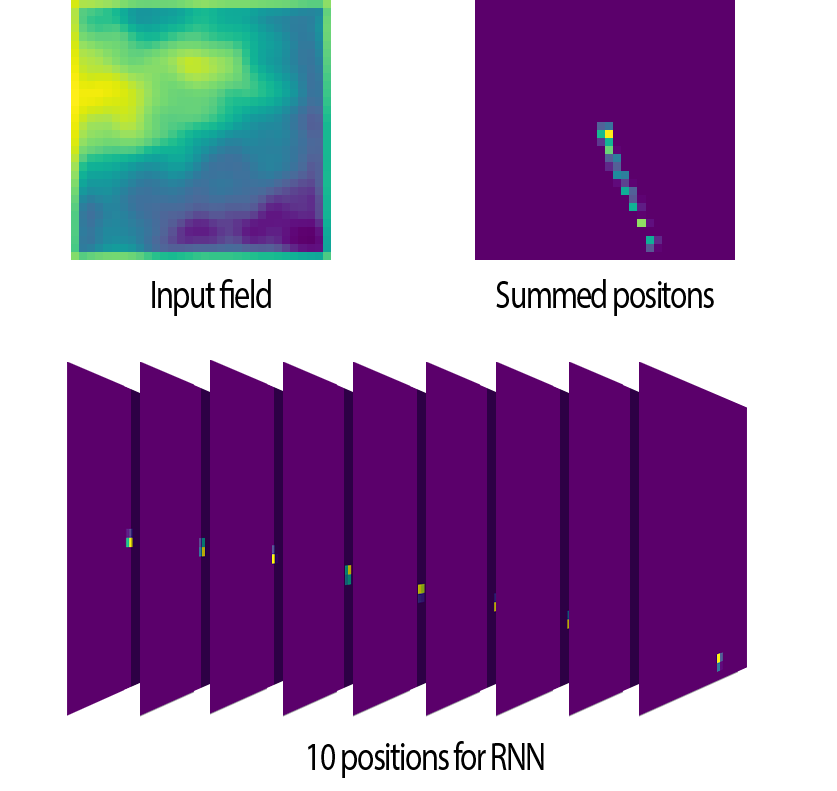
\includegraphics[width=0.7\textwidth]{Figures/Positions_vis.png}
    \caption{Data provided to our models. The particle trajectory is either encoded by summing all the four-warm positions in one field, as illustrated in the top right, or as separate fields used supplied to each time step of a recurrent network, as shown at the bottom of the figure.}
    \label{fig:position_input}
\end{figure}

\subsection{Model}
% Present our model implementations
Our models are implemented using the Keras API in TensorFlow. It gives us a simple and flexible way of implementing neural networks. In the results we present the results of four final model architectures. Going from simple to complicated, we have a standard dense neural network (DNN) without any bells or whistles, a convolutional neural network (CNN) that will hopefully understand the spatial part well, a recurrent neural network that should grasp the temporal dimension of our problem, and a convolutional recurrent neural network (CRNN) that we expect to handle it all. These models are illustrated in figure \ref{fig:model_graph}. The DNN and CNN models are straight forward to implement using Keras' Sequential API, but the CRNN model is more complicated, so we cover in detail how it is implemented later. Because we have unlimited data all models are trained with only one epoch with the desired batches. This prevents overfitting and memorization of specific input data and therefore will likely make models perform better on unseen data.

\begin{figure}
    \centering
    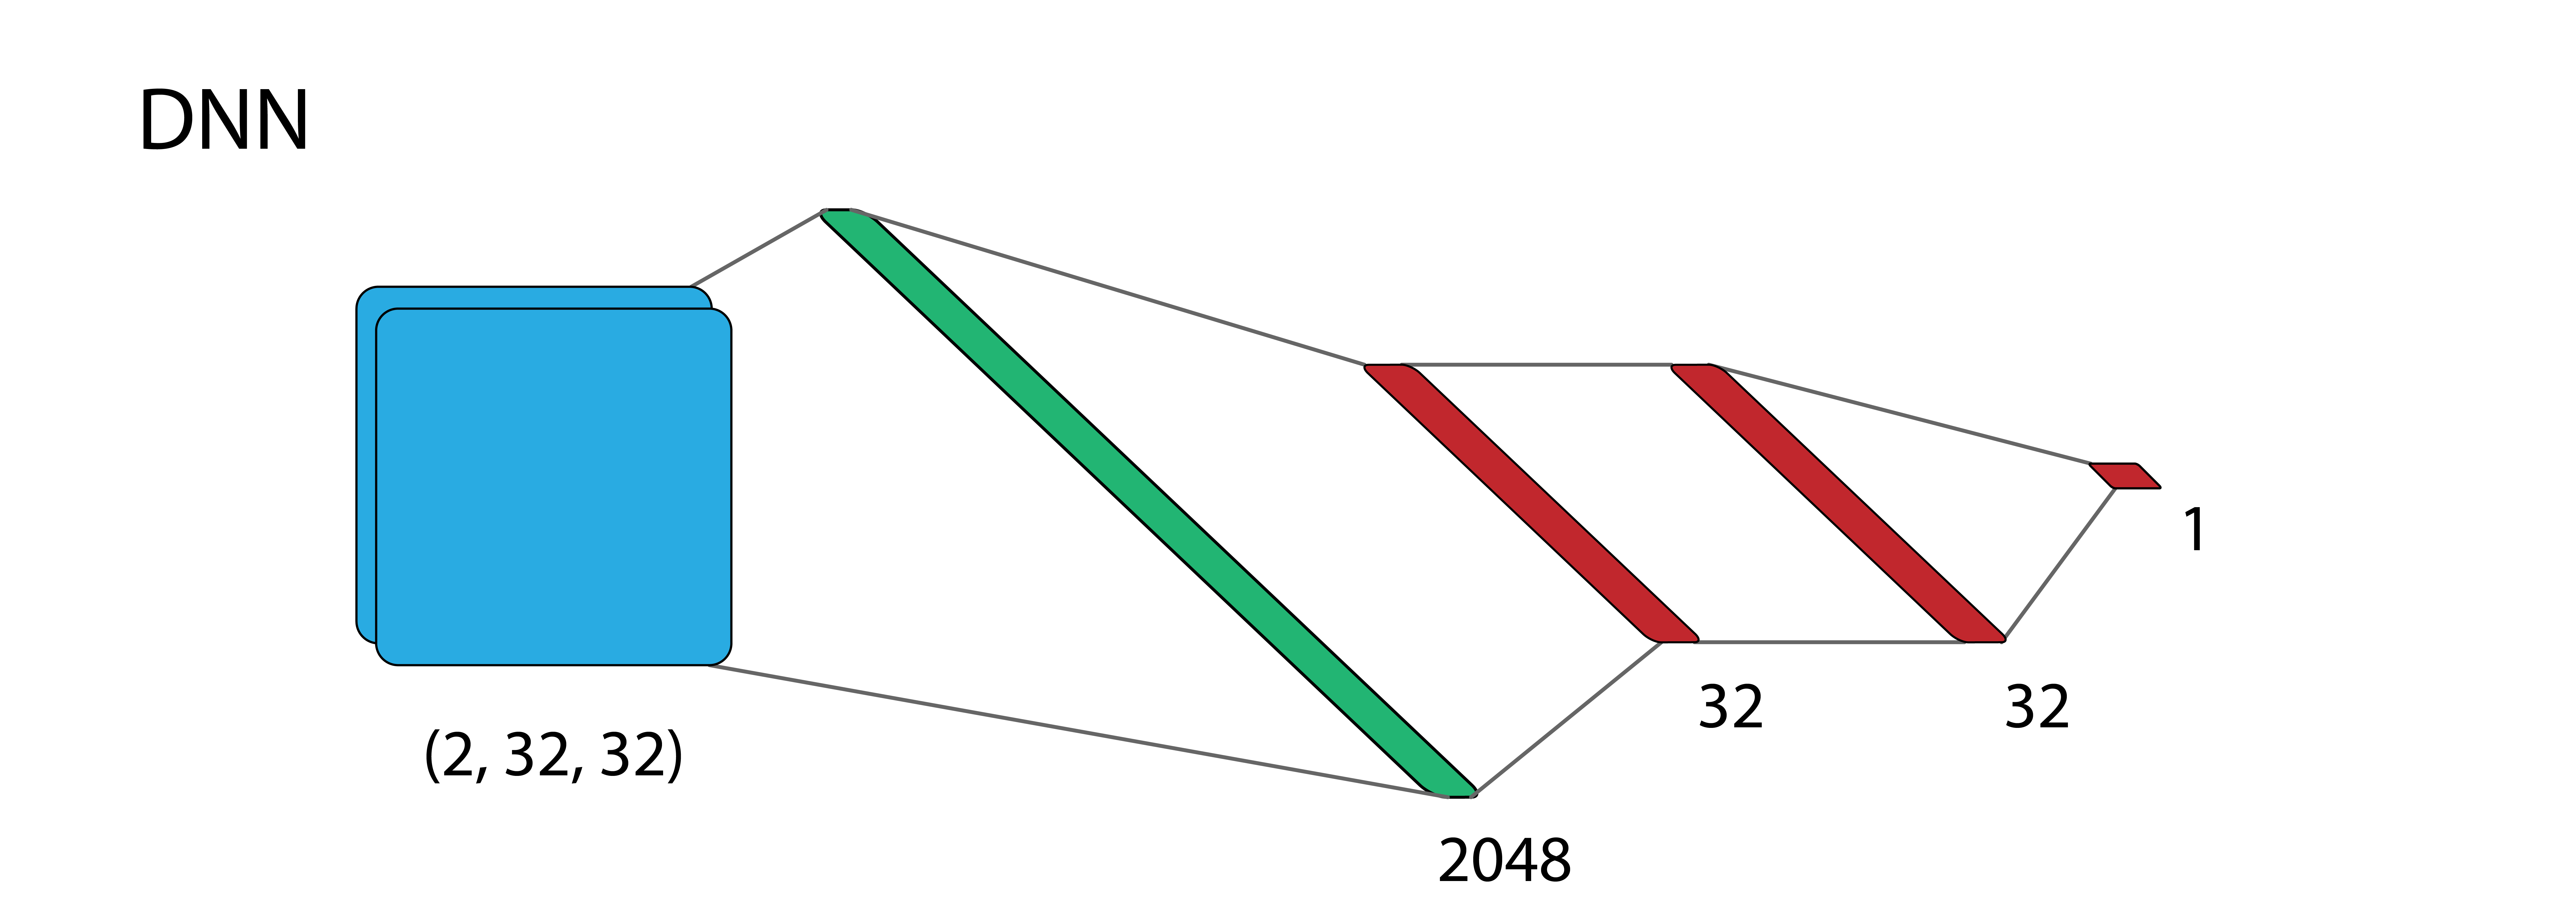
\includegraphics[width=0.9\textwidth]{Figures/DNN_1.png}
    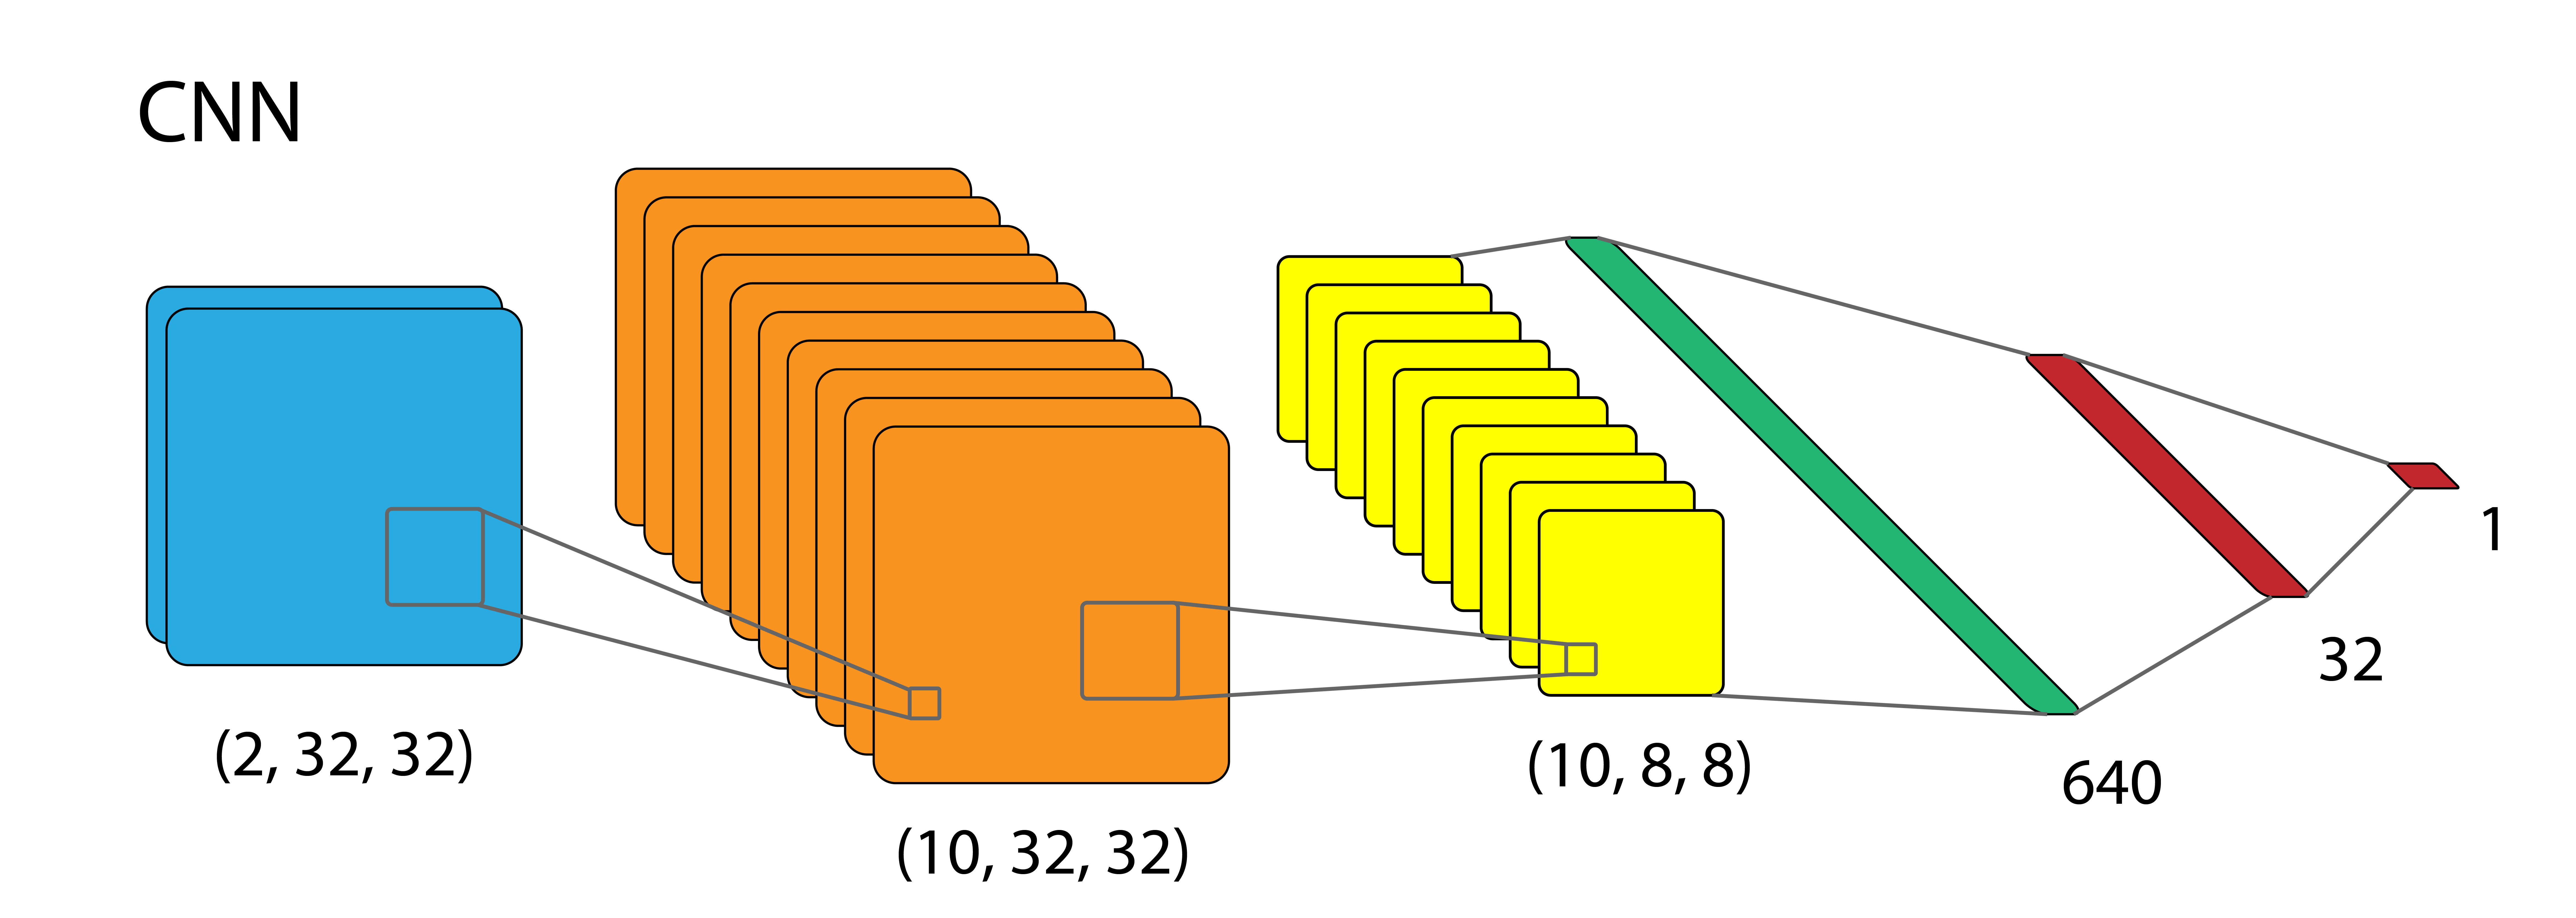
\includegraphics[width=0.9\textwidth]{Figures/CNN_1.png}
    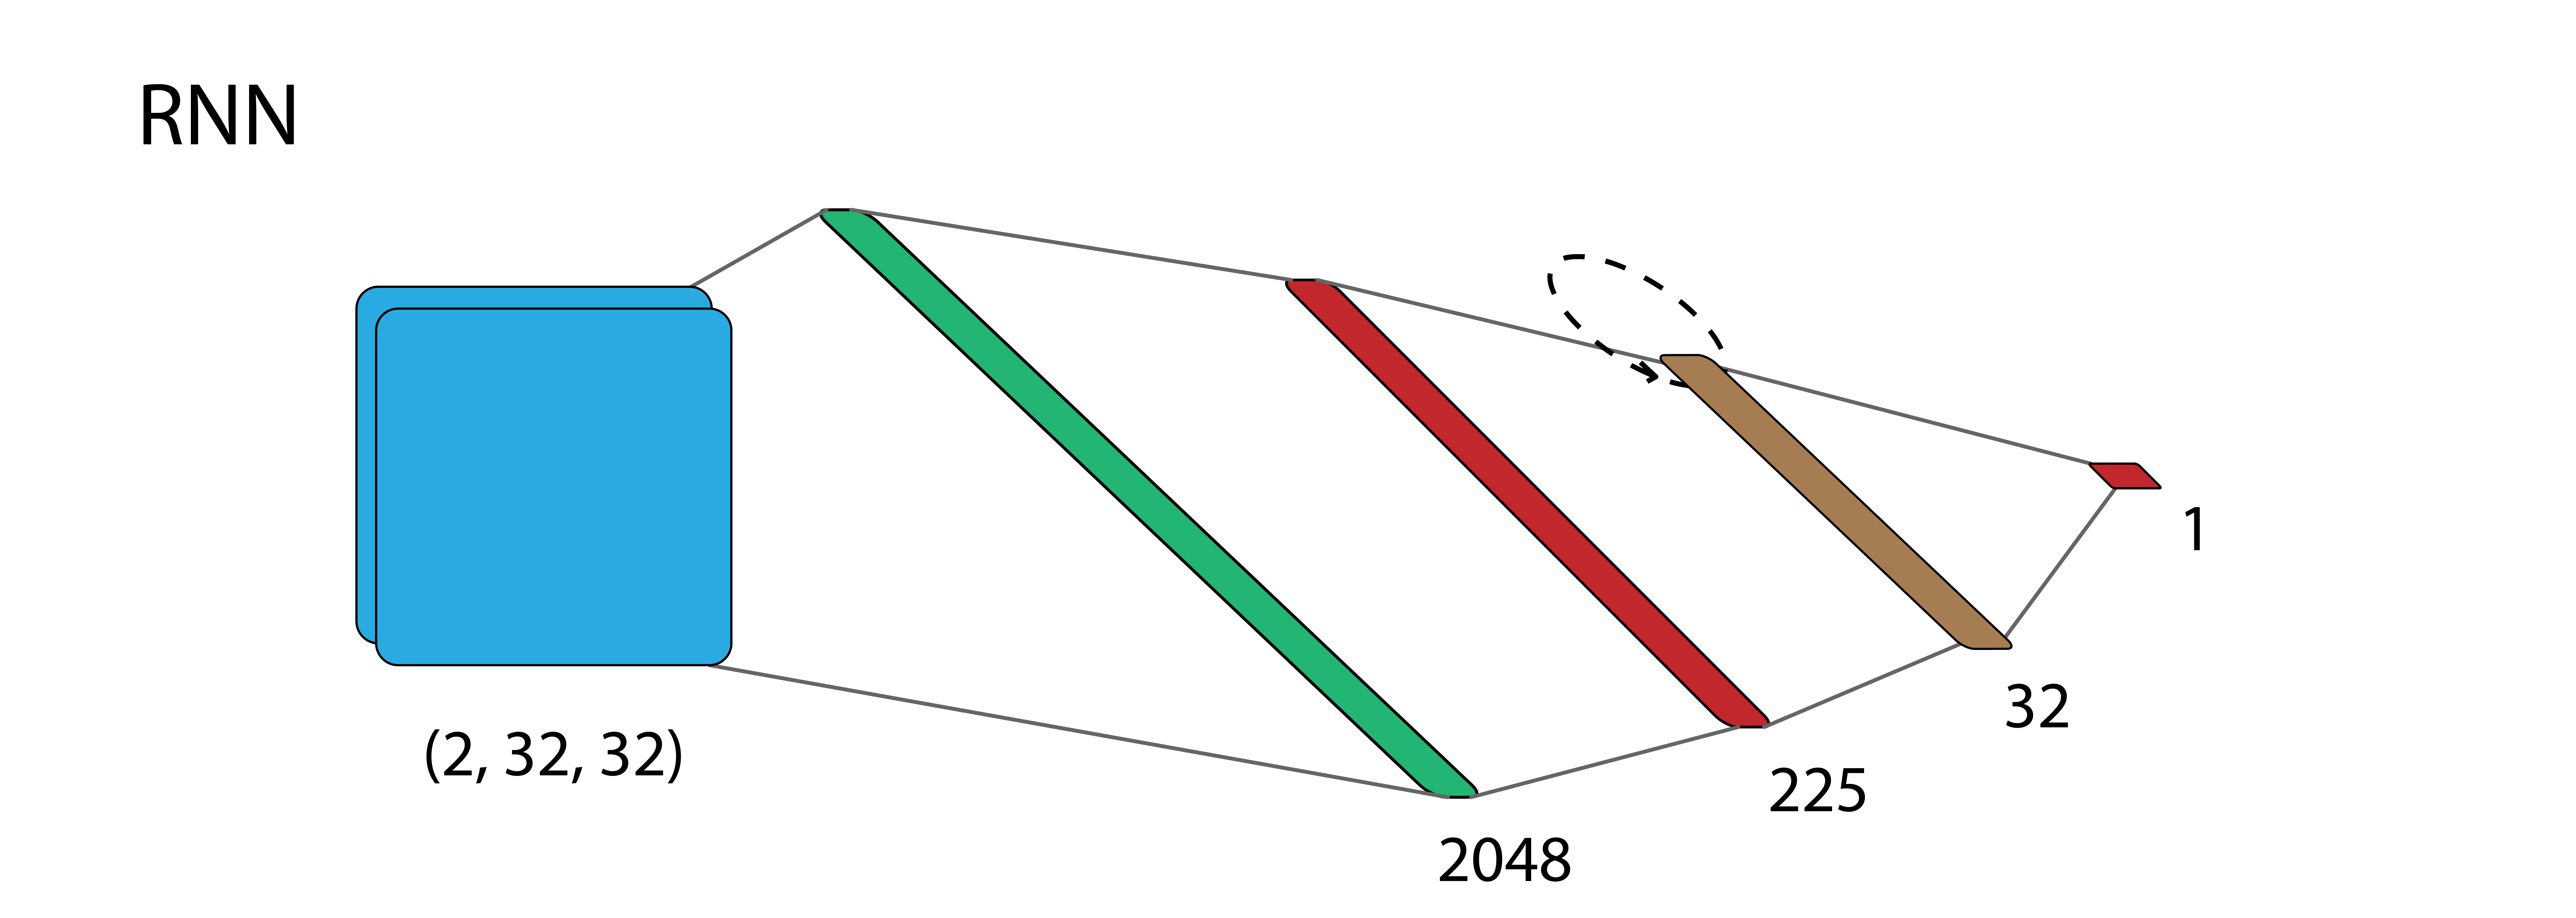
\includegraphics[width=0.9\textwidth]{Figures/RNN.png}
    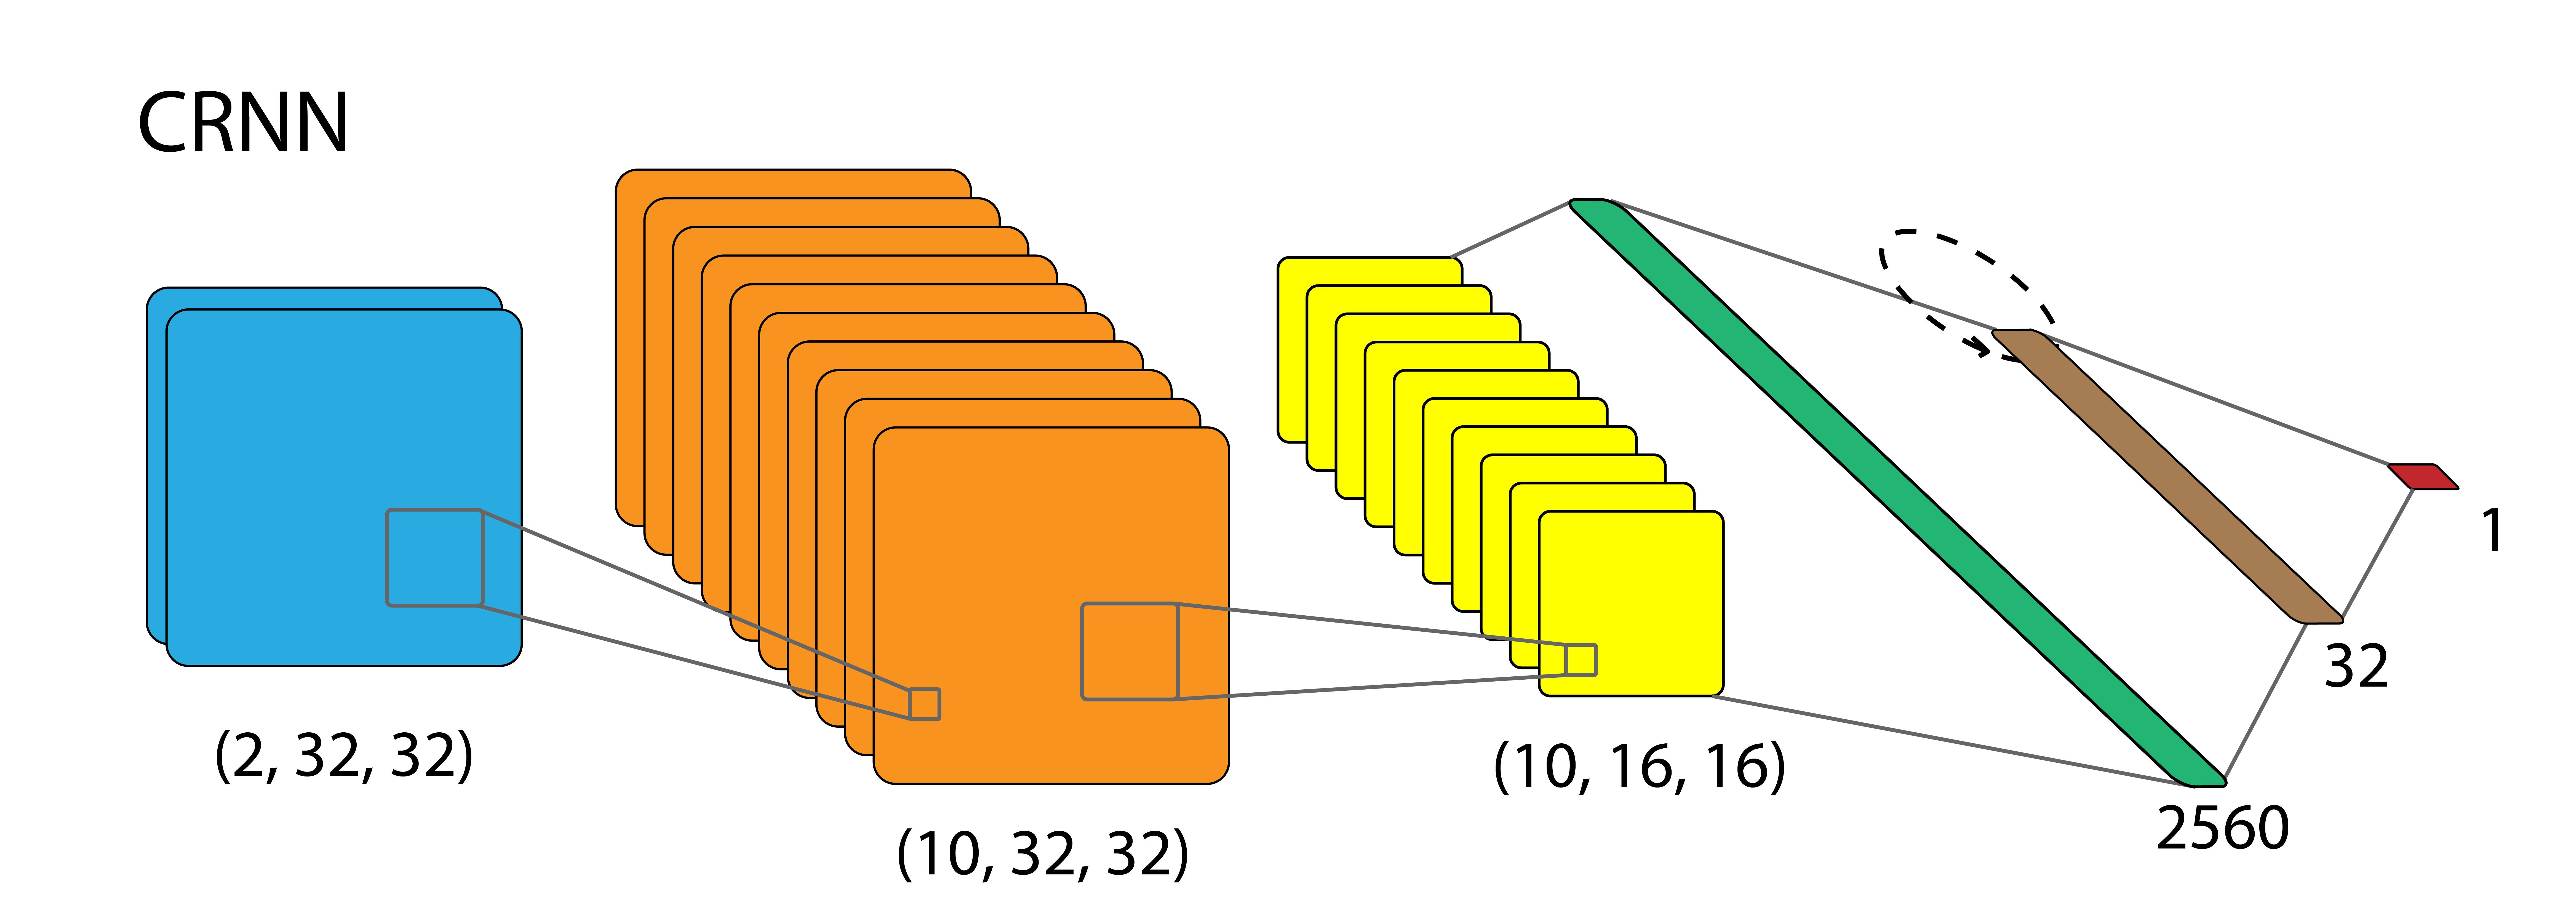
\includegraphics[width=0.9\textwidth]{Figures/CRNN_1.png}
    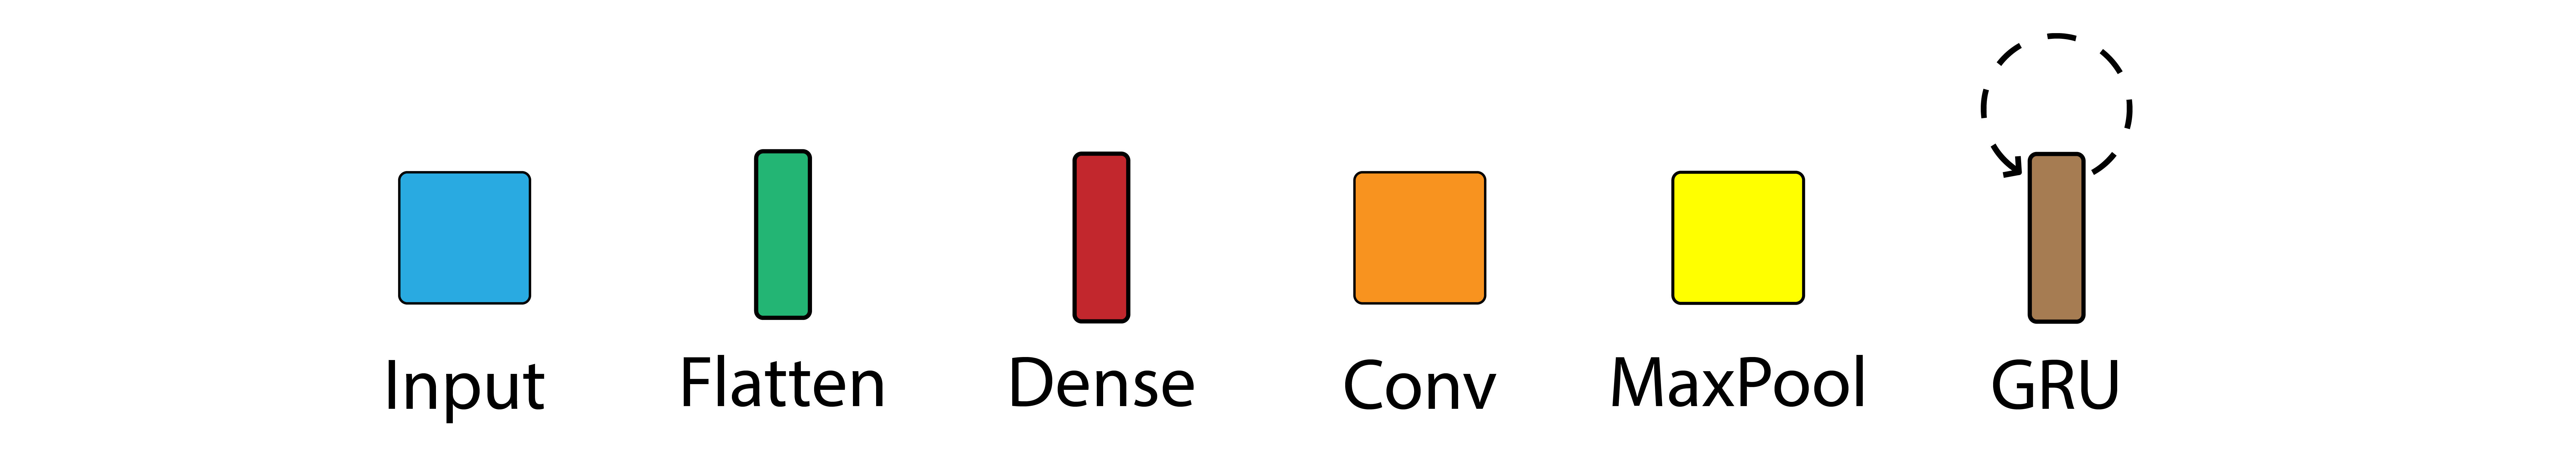
\includegraphics[width=0.9\textwidth]{Figures/model_legend2.png}
    \caption{The four models used in this project. The two blue input squares represent the position and the field. Multiple convolutional squares represent multiple filters producing multiple channels which results in multiple channels in the MaxPool layers as well.}
    \label{fig:model_graph}
\end{figure}

\subsubsection{Recurrent and convolutional recurrent networks}

We want to test the performance of recurrent neural networks with a convolutional part, and without a convolutional part. Because our implementations for both of these cases are very similar, and they are being fed data in the same way, we have combined them into one class. The challenge with implementing both of them, if we're going to use the training algorithm described in section \ref{subsubsec:crnn_theory}, is that we somehow have to embed the time dimension spatially. This cannot be done by using the Sequential API alone. We have therefore subclassed the Keras Model class, and overwritten the call method, as given in listing \ref{lst:convolution-call}.

\begin{lstlisting}[
  caption={The \lstinline{call} method of our Keras Model subclass},
  float,
  language=Python,
  label={lst:convolution-call}
]
def call(self, batches, **kwargs):
    """Custom call method for making batch predictions.

    :param batches: Arraylike with shape (batches, *self.spatial_input_shape).
    :param **kwargs: Ignored. Only here for compatibility.

    :return: tf.Tensor object with predictions for each batch.
    """
    num_batches = batches.shape[0] or 1
    predictions = []
    for i in range(num_batches):
        spatial = self.spatial(batches[i])
        # time_major==True => GRU expects data on format [timesteps, batches, predictors]
        gru, _ = self.gru(spatial[:, np.newaxis])
        predictions.append(self.prediction(gru))

    return tf.convert_to_tensor(predictions)
\end{lstlisting}

In our call method, the \lstinline{batches} input we take in has the dimensions \lstinline{(batch, time steps, x, y, channels)}. This means we have made the tensor of one higher order than is normal, and have hijacked what is usually the batch part of the Conv2D input of Keras, and used it for time steps. We thus need to iterate over the batches in pure Python, and likely miss out on lots of Tensorflow performance.

The class subclassed from tf.keras.Model then has two factory methods, one for creating a CRNN, and one for RNN with dense layers to attempt to solve the spatial part. In addition to this model class, we have built an agent class for training and testing the model, building batches for both of them, and plotting the results.

\section{Results}

\subsection{Feed forward neural networks}
Both the convolutional and dense networks achieved promising results when predicting based on the trajectory of the particle. In the first iteration of the models we only gave them the final position, but then the models converged to predict the mean mass similar to what we see in figure \ref{fig:rnn-results}.

The CNN model performs slightly better than the DNN. Their predictions are shown in figure \ref{fig:pred_cnn_dnn}. Figure \ref{fig:hist_cnn_dnn} shows scores for 40 separate training runs of the models, revealing that the CNN in general performs better and has more consistent training. However, 11 of the trained CNN models are discarded due to them not learning anything and just predicting zero. The CNN model is very sensitive to small changes in the initial parameters and about 25\% of the training runs result in the model only predicting 0 for every input. In the early stages we used a more complex model where this occurred in about half the runs. Neither model has fully converged after 6000 batches as seen in figure \ref{fig:train_cnn_dnn} which suggests that they can improve further with more training.

\begin{figure}
    \centering
    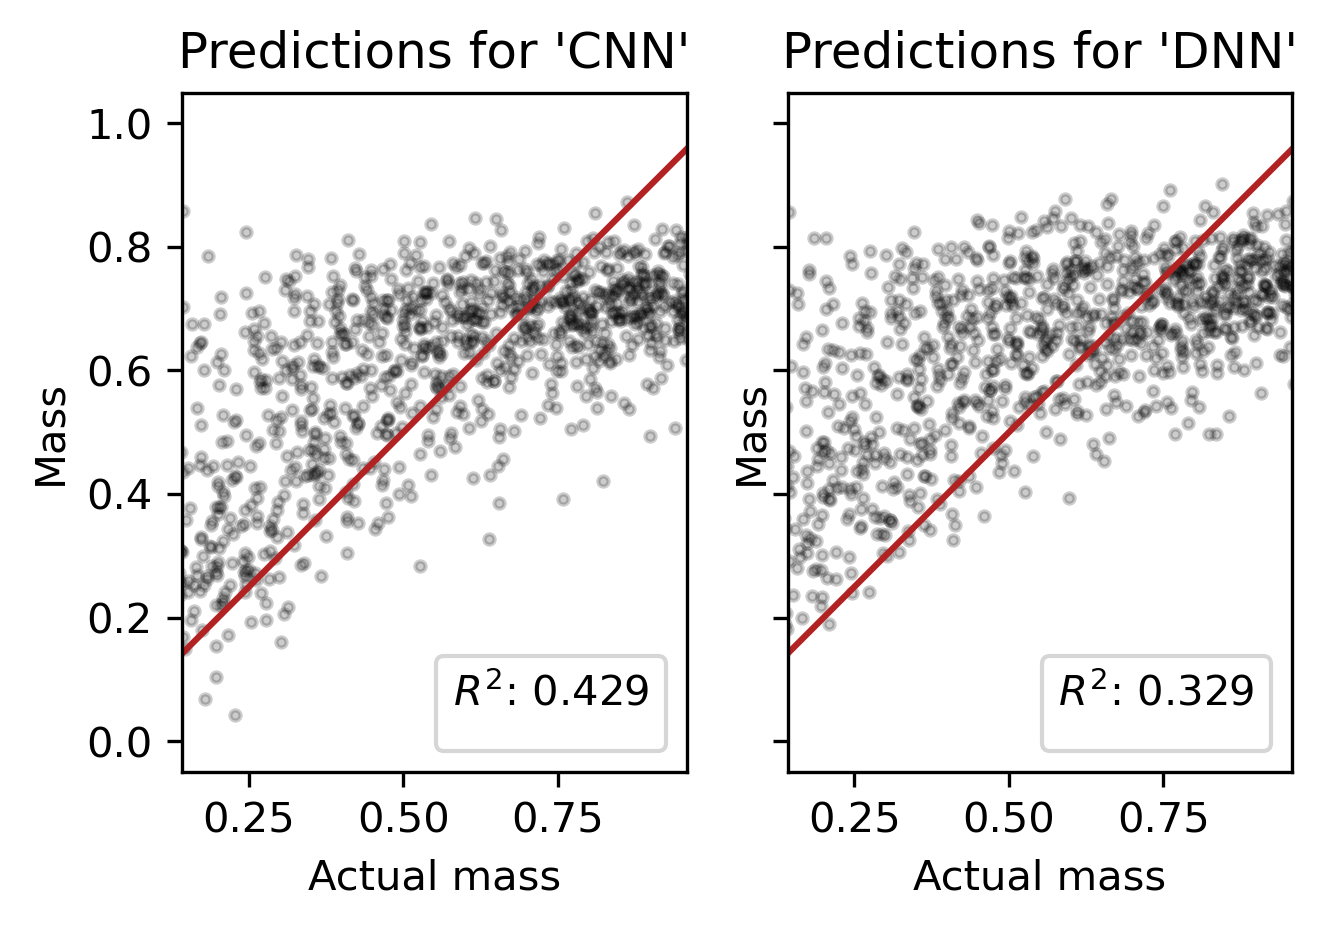
\includegraphics[width=0.8\textwidth]{Figures/predictions_cnn_dnn.png}
    \caption{Predictions made by the CNN and DNN models after training on 14 000 particle simulations. The red line marks what would have been correct predictions. Points under the red line means the model predicted a too low mass, while points over the red line means the prediction was too high.}
    \label{fig:pred_cnn_dnn}
\end{figure}

\begin{figure}
    \centering
    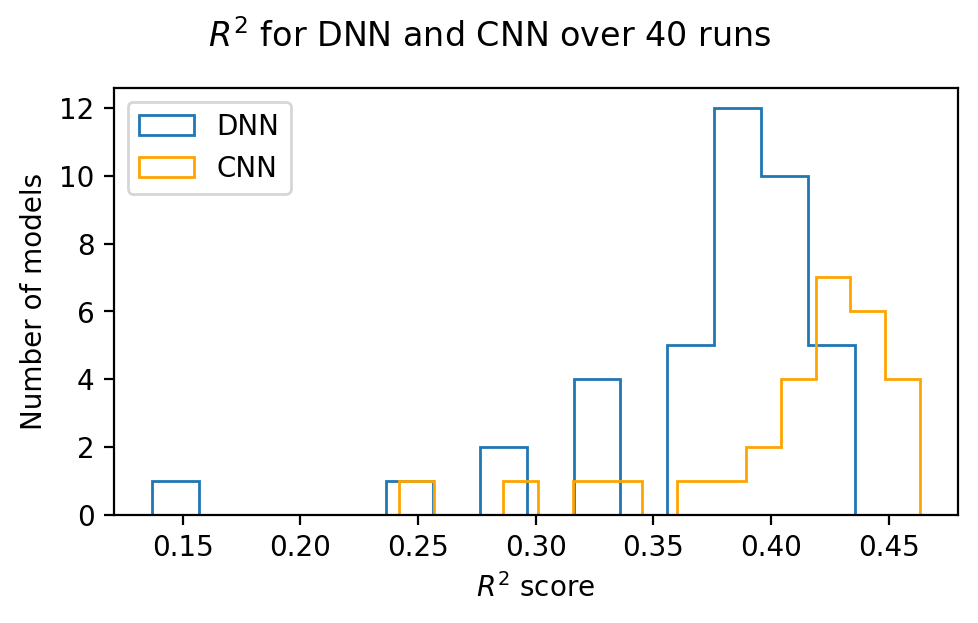
\includegraphics[width=0.8\textwidth]{Figures/dnn_cnn_hist.png}
    \caption{Distribution of $R^2$ scores for 40 training runs of the DNN and CNN models. 11 of the CNN models are discarded from the plot as outliers, they achieved $R^2 = -4.77$ which corresponds to predicting just zeros.}
    \label{fig:hist_cnn_dnn}
\end{figure}

\begin{figure}
    \centering
    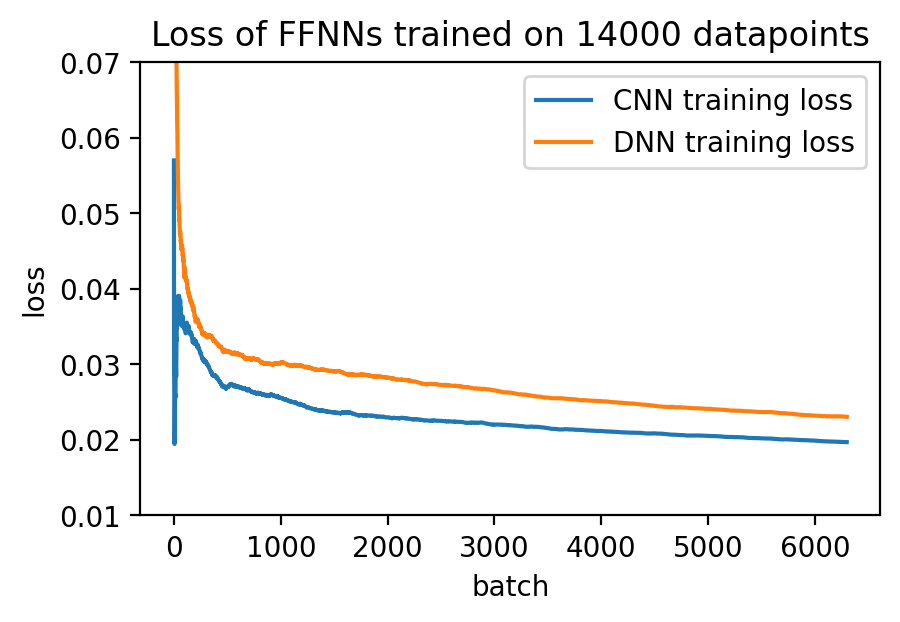
\includegraphics[width=0.8\textwidth]{Figures/train_dnn_cnn.png}
    \caption{Loss history of the CNN and DNN models. Each batch contains two particle simulations. The CNNs train faster, but both improve throughout the entirety of the training which suggests they might converge towards the same loss eventually.}
    \label{fig:train_cnn_dnn}
\end{figure}

\subsection{Recurrent neural network}

The purely recurrent neural network, without any convolutional part, performs poorly on our problem. As seen in fig \ref{fig:rnn-results}, it only tends towards the average. This is likely due to the data being complicated and large, and to it being difficult unravelling the spatial aspect and what is what, without either convolutions or encoding in a less data-heavy way. If we were to encode it as we have done with the DNN and CNN, there would no longer be any use for the recurrent part, since it would all be the same time step. We write this to make it clear that the RNN didn't perform worse than the DNN on the same data, just that there was a clever way of dealing with the data that made recurrence obsolete.

\begin{figure}
    \centering
    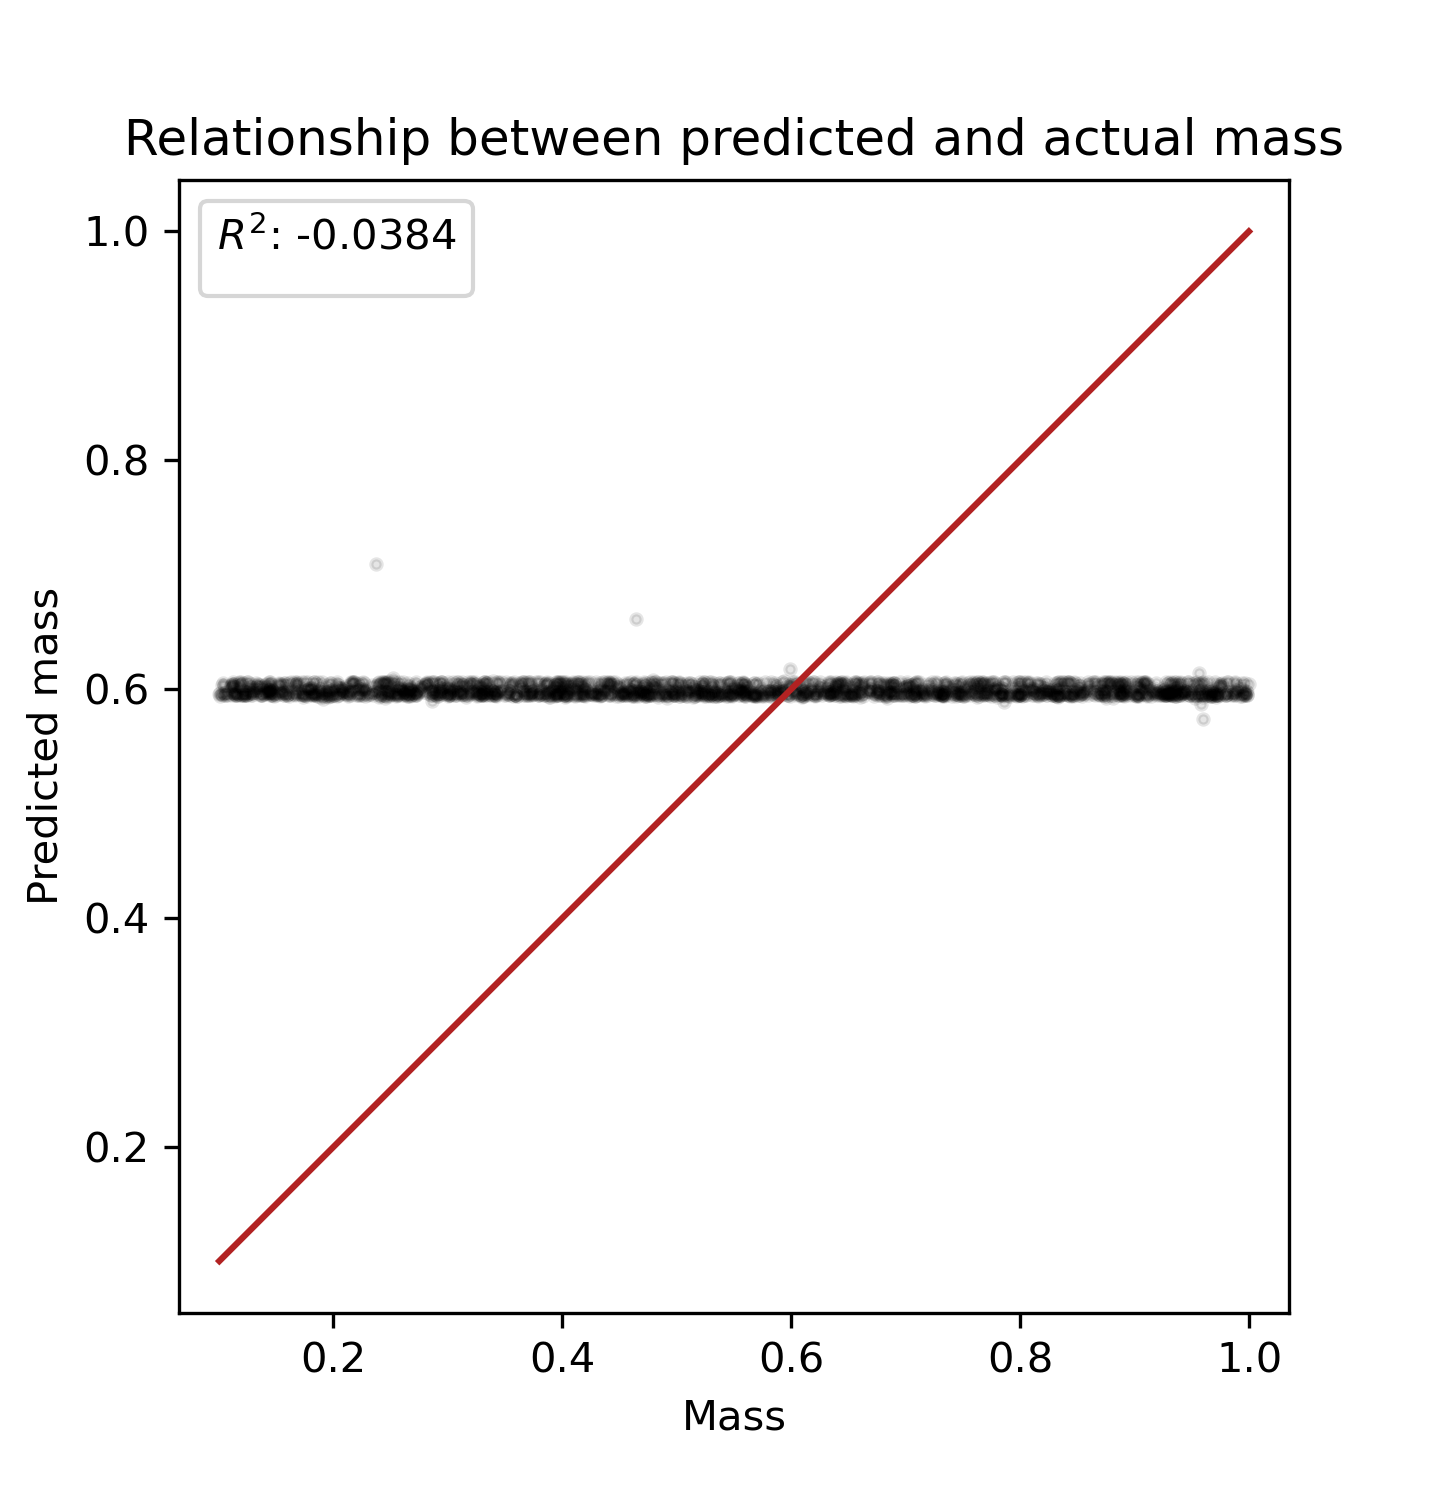
\includegraphics[width=0.8\textwidth]{Figures/rnn_results.png}
    \caption{Results after training the pure recurrent neural net on 5000 batches. On the x axis is the actual mass, and on the y axis the predicted mass. The red diagonal line indicate perfect predictions, while the dots indicate the predictions the model made. There is little correlation between these two, in fact the Pearson correlation coefficient between the actual and predicted mass is only roughly $0.018$.}
    \label{fig:rnn-results}
\end{figure}

There has been very little effort put into tuning this model. The model just has three layers; one dense, one GRU, and another dense one with just the prediction.

The RNN and the DNN discussed above are quite similar, but the DNN solves the problem a lot better. The aspect that differentiates the RNN from the DNN, and is responsible for this difference in performance, is that the RNN takes in the time steps one by one, and is supposed to store the important information in between steps. The DNN on the other side takes in the positions from all the different time steps summed once. The data the RNN receives is probably too chaotic and large for it to be able to train to. Dropout could very possibly reduce this problem, but as mentioned before, we haven't looked into it or any other regularisation.

\subsection{Convolutional recurrent neural network}

Our most complicated model, with both a convolutional and a recurrent part, performs well on our problem. In figure \ref{fig:crnn-results}, you can see how it trains, and what the predictions look like after training. Let us discuss these three subplots one by one.

\begin{figure}
    \centering
    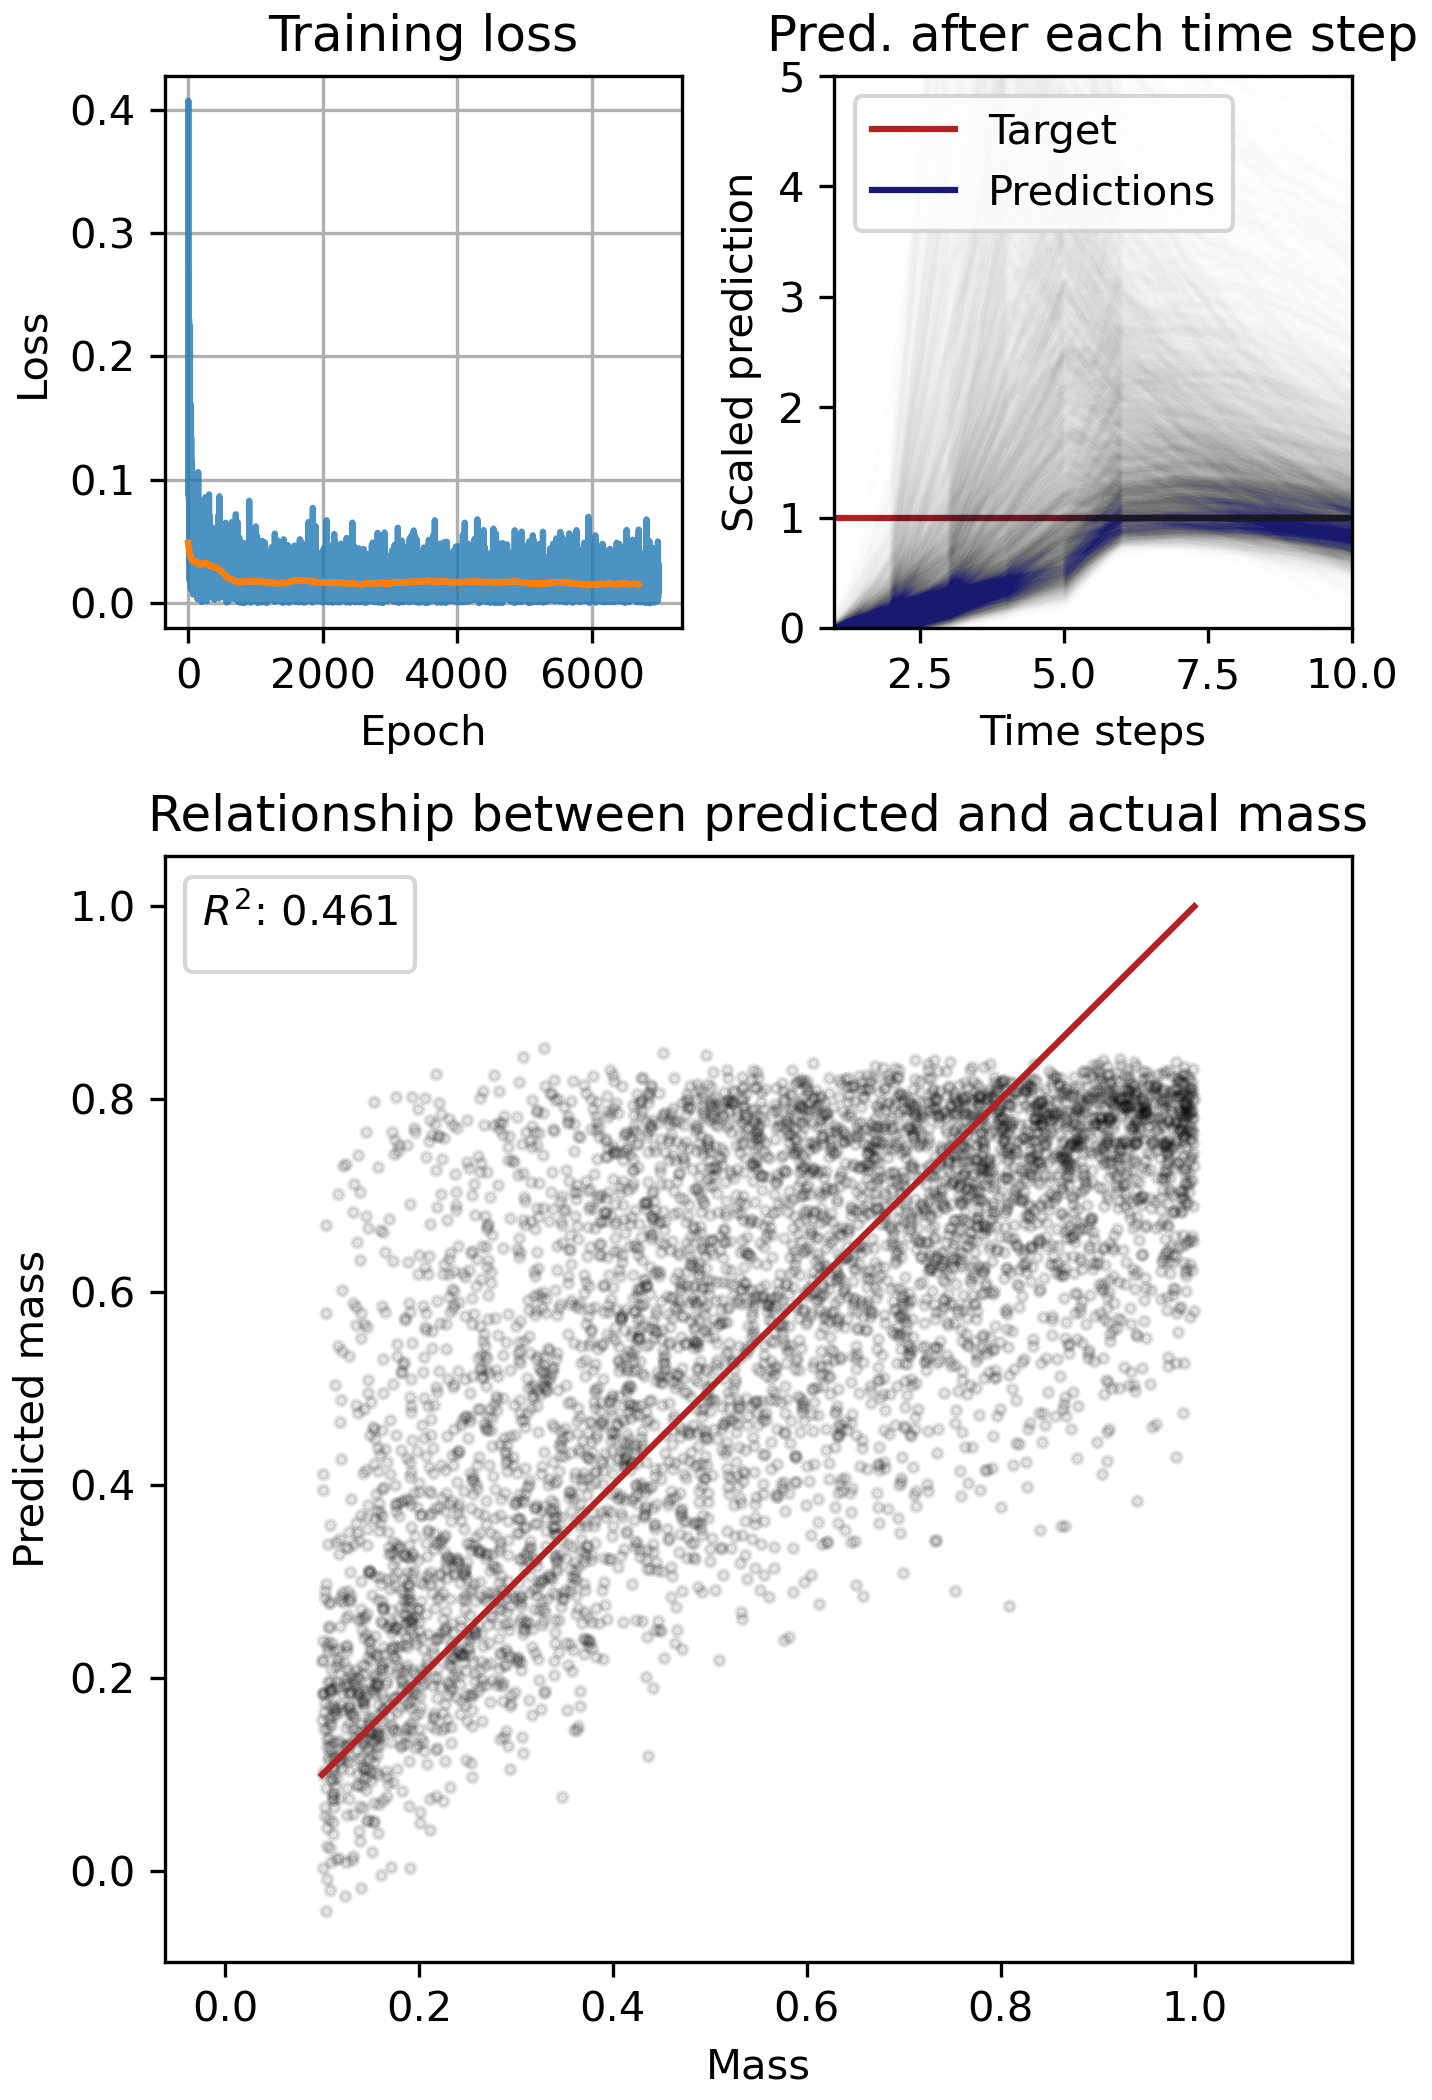
\includegraphics[width=0.8\textwidth]{Figures/crnn_results_10.png}
    \caption{Results after training the convolutional recurrent neural net on 7000 epochs with 3 batches in each. In the top left plot, we see the training loss, with the blue lies being from each batch, and the red being a rolling average. The top right plot shows how the prediction of each case changes over time. Each line is one mass, and the height is what prediction is made at that time step, divided by the actual mass. This means that $1$ is the correct answer for all the lines. The large, bottom plot indicates the relationship between end predictions, and the actual masses. If the model was perfect, all predictions would lie on the red line. For the test shown in that plot, the Pearson correlation coefficient was $0.690$}
    \label{fig:crnn-results}
\end{figure}

As seen in the top left subplot of figure \ref{fig:crnn-results}, training seems to be very unstable, and also doesn't seem to make much difference after roughly 1000 batches. The instability comes from having only 3 samples per gradient descent step. We need this stochastisity because we have no regularisation, and our complicated model only converges to predict the average mass if we give it more than roughly 3 batches at a time. The small difference in loss from untrained to trained comes from our loss function not being optimal. As discussed in section \ref{subsec:loss_theory}, we have looked at three different loss functions, but none of them were perfect.

In the top right subplot, it is evident that the majority of the predictions follow the same relatively smooth curve ending up somewhere near $1$. This is good, and shows that the temporal data is being put to use - it can't immediately tell the mass, it adjusts over time when new data is made available. We also see that the model often overshoots drastically in the beginning, but that it eventually converges towards the actual mass. It does however not seem like just giving it more time steps would make the estimates get much better.

For some reason, all estimates, not only those that are higher than the actual mass, have a tendency to shrink over time (see the thicker blue line from time step 8 and outwards). This is general, and not only a random artifact in this specific model, and we have no good explanation for it.

One thing to note about the predictions after every time step, is that we haven't trained the model to give them. As discussed in section \ref{subsubsec:crnn_theory}, during training we only look at and fit based on the end prediction. The predictions we have extracted after $n$ time steps does therefore not necessarily match the prediction a model trained on making a prediction after $n$ time steps. It is very possible that the model has learned how many time steps it has to make the prediction, and stores data differently based on what time step it is in.

In the main plot of figure \ref{fig:crnn-results}, we can see that our prediction clearly has some relation to the target. The concentration of predictions is higher around the red optimal line, than above or below it. The $R^2$ score is $0.461$, which is the highest obtained by any of the models in the report. However, these models all vary a lot, and we don't have enough data to be entirely sure that this architecture is the best.

A big issue with our predictions is that it never predicts the highest values for the mass. We have tested for different ranges of masses, and whatever range we choose, the top roughly $15\%$ of the range is never predicted with these parameters. Other kernel sizes grant different cutoffs, and for some kernel sizes this problem has only occurred in the purely convolutional neural network. Why this happens is an open question, and it very well could be that it is just a good strategy for getting less loss. This because tending towards the average when the values are extreme is less risky, but if this was the case, the cutoff should be symmetric.

\subsection{Model comparison}
As shown in table \ref{tab:model_comparison}, the convolutional-recurrent model outperforms the others the others with some margin. The convolutional and dense models follow as second and third best, while the recurrent model, which only learns the mean of the mass distribution, performs worst. The differences are not as big as we might have hoped for, but we believe the restricted training time is partly to blame. The recurrent models are significantly more complex than the feed-forward models, and would likely benefit from training on larger data sets and for a longer time.

\begin{table}
    \centering
    \caption{$R^2$-scores for our dense, convolutional and convolutional-recurrent neural network models.}
    \begin{tabular}{c  c  c}
    Model & $R^2$-score \\
    \hline
    DNN  & 0.373 \\
    CNN  & 0.408 \\
    RNN  & -0.038 \\
    CRNN & 0.461
    \end{tabular}
    \label{tab:model_comparison}
\end{table}

\section{Conclusion}
The main aim of this project was to develop neural networks that achieve a general understanding of how particles move in force fields based on their mass, and then predict the particle's mass. The models showed promising results but we expect that they can be improved further. Using the field and ten separate arrays to represent the position, the best model, with both convolution and recurrence, was routinely able to make predictions with $R^2=0.461$ on unseen data.

Feed forward neural networks with and without convolution are also able to solve the problem with purely dense networks achieving an average of $R^2=0.373$ and with convolutional layers reaching $R^2= 0.408$. However, the convolutional layers are quite unstable and often produce non-functional models about 25\% of the time. 

The convolutional recurrent network slightly outperforms the two simpler models, but has 10 times as many parameters. For this problem complexity is not necessarily an issue as it is difficult to overfit the models when using an endless stream of synthetic data. However, the results most likely do not extrapolate to significantly different fields or bigger masses. 

\subsection{Future research}
Moving forward the next steps would likely be developing systematic model tuning and possibly configurations to the dataset. 

Most of the work on this project revolved around making the models understand the data and developing the more complicated CRNN model. The lack of systematic tuning of the models is likely the biggest limiting factor of our results. In early development we explored a set of hyperparameters, but a whole project can be developed around tuning the models. Possible developments here include dropout and regularization of the convolutional recurrent models, and exploring more model architectures beyond the four presented here and the ones we looked at in early development. 

The problem can be developed further by adding multiple force fields acting on the particles simultaneously. This way, the particle's acceleration at any time step might be determined by its charge, drag coefficient, mass, gravity, magnetism, the air pressure, and/or wind fields. It would also be possible to exclude the gravity field, and have the gravity be constant in space and time (either zero or nonzero), thus making the mass more implicit. Fields can also change over time or only have sparse data points. Complicating the problem is however only a reasonable development after developing models that predict well on the simpler problem discussed in this project.

A data development that is compatible with the models presented in the project is creating more realistic data. The fields used in this project are generated using Perlin noise and there are walls along the perimeter to keep the particle within the boundaries of the field. It is possible that these fields do not sufficiently approximate realistic fields. Real world data or spending more time developing the fields themselves might make the models more relevant to real world applications.



\printbibliography

\end{document}
